\documentclass[11pt,a4paper,oneside]{report}             % Single-side
%\documentclass[11pt,a4paper,twoside,openright]{report}  % Duplex

%\PassOptionsToPackage{chapternumber=Huordinal}{magyar.ldf}
\usepackage{t1enc}
\usepackage[latin2]{inputenc}
\usepackage{amsmath}
\usepackage{amssymb}
\usepackage{enumerate}
\usepackage[thmmarks]{ntheorem}
\usepackage{graphics}
\usepackage{epsfig}
\usepackage{listings}
\usepackage{color}
%\usepackage{fancyhdr}
\usepackage{lastpage}
\usepackage{anysize}
\usepackage[magyar]{babel}
\usepackage{sectsty}
\usepackage{setspace}  % Ettol a tablazatok, abrak, labjegyzetek maradnak 1-es sorkozzel!
\usepackage[hang]{caption}
\usepackage{subcaption}
\usepackage{hyperref}
\usepackage{pgfplots}
\usepackage{tikz}
\usepackage[miktex]{gnuplottex}
\usepackage{pgfplotstable}


%--------------------------------------------------------------------------------------
% Main variables
%--------------------------------------------------------------------------------------
\newcommand{\vikszerzo}{Nyitrai J�zsef}
\newcommand{\vikkonzulens}{Juh�sz Zolt�n}
\newcommand{\vikcim}{Sz�kelyf�ld �nekes �s hangszeres zenekult�r�j�ban rejl� ritmikai �sszef�gg�sek vizsg�lata}
\newcommand{\viktanszek}{Sz�m�t�studom�nyi �s Inform�ci�elm�leti Tansz�k}
\newcommand{\vikdoktipus}{Diplomaterv}
\newcommand{\vikdepartmentr}{Nyitrai J�zsef}

%--------------------------------------------------------------------------------------
% Page layout setup
%--------------------------------------------------------------------------------------
% we need to redefine the pagestyle plain
% another possibility is to use the body of this command without \fancypagestyle
% and use \pagestyle{fancy} but in that case the special pages
% (like the ToC, the References, and the Chapter pages)remain in plane style

\pagestyle{plain}
%\setlength{\parindent}{0pt} % �ttekinthet�bb, angol nyelv� dokumentumokban jellemz�
%\setlength{\parskip}{8pt plus 3pt minus 3pt} % �ttekinthet�bb, angol nyelv� dokumentumokban jellemz�
\setlength{\parindent}{12pt} % magyar nyelv� dokumentumokban jellemz�
\setlength{\parskip}{0pt}    % magyar nyelv� dokumentumokban jellemz�

\marginsize{35mm}{25mm}{15mm}{15mm} % anysize package
\setcounter{secnumdepth}{0}
\sectionfont{\large\upshape\bfseries}
\setcounter{secnumdepth}{2}
\singlespacing
\frenchspacing

%--------------------------------------------------------------------------------------
%	Setup hyperref package
%--------------------------------------------------------------------------------------
\hypersetup{
    bookmarks=true,            % show bookmarks bar?
    unicode=false,             % non-Latin characters in Acrobat�s bookmarks
    pdftitle={\vikcim},        % title
    pdfauthor={\vikszerzo},    % author
    pdfsubject={\vikdoktipus}, % subject of the document
    pdfcreator={\vikszerzo},   % creator of the document
    pdfproducer={Producer},    % producer of the document
    pdfkeywords={keywords},    % list of keywords
    pdfnewwindow=true,         % links in new window
    colorlinks=true,           % false: boxed links; true: colored links
    linkcolor=black,           % color of internal links
    citecolor=black,           % color of links to bibliography
    filecolor=black,           % color of file links
    urlcolor=black             % color of external links
}

%--------------------------------------------------------------------------------------
% Set up listings
%--------------------------------------------------------------------------------------
\lstset{
	basicstyle=\scriptsize\ttfamily, % print whole listing small
	keywordstyle=\color{black}\bfseries\underbar, % underlined bold black keywords
	identifierstyle=, 					% nothing happens
	commentstyle=\color{white}, % white comments
	stringstyle=\scriptsize\sffamily, 			% typewriter type for strings
	showstringspaces=false,     % no special string spaces
	aboveskip=3pt,
	belowskip=3pt,
	columns=fixed,
	backgroundcolor=\color{lightgray},
} 		
\def\lstlistingname{lista}	

%--------------------------------------------------------------------------------------
%	Some new commands and declarations
%--------------------------------------------------------------------------------------
\newcommand{\code}[1]{{\upshape\ttfamily\scriptsize\indent #1}}

% define references
\newcommand{\figref}[1]{\ref{fig:#1}.}
\renewcommand{\eqref}[1]{(\ref{eq:#1})}
\newcommand{\listref}[1]{\ref{listing:#1}.}
\newcommand{\sectref}[1]{\ref{sect:#1}}
\newcommand{\tabref}[1]{\ref{tab:#1}.}

\DeclareMathOperator*{\argmax}{arg\,max}
%\DeclareMathOperator*[1]{\floor}{arg\,max}
\DeclareMathOperator{\sign}{sgn}
\DeclareMathOperator{\rot}{rot}
\definecolor{lightgray}{rgb}{0.95,0.95,0.95}

\author{\vikszerzo}
\title{\viktitle}
\includeonly{
	%guideline,%
	%project,%
	titlepage,%
	declaration,%
	abstract,%
	introduction,%
	chapter1,%
	chapter2,%
	chapter3,%
	acknowledgement,%
	appendices,%
}
%--------------------------------------------------------------------------------------
%	Setup captions
%--------------------------------------------------------------------------------------
\captionsetup[figure]{
%labelsep=none,
%font={footnotesize,it},
%justification=justified,
width=.75\textwidth,
aboveskip=10pt}

\renewcommand{\captionlabelfont}{\small\bf}
\renewcommand{\captionfont}{\footnotesize\it}

\usepgfplotslibrary{groupplots}
\usetikzlibrary{patterns}

%--------------------------------------------------------------------------------------
% Table of contents and the main text
%--------------------------------------------------------------------------------------
\begin{document}
\singlespacing
%\include{guideline}
%%--------------------------------------------------------------------------------------
% Feladatkiiras (a tanszeken atveheto, kinyomtatott valtozat)
%--------------------------------------------------------------------------------------
\clearpage
\begin{center}
\large
\textbf{FELADATKI�R�S}\\
\end{center}

A feladatki�r�st a tansz�ki adminisztr�ci�ban lehet �tvenni, �s a leadott munk�ba eredeti, tansz�ki pecs�ttel ell�tott �s a tansz�kvezet� �ltal al��rt lapot kell belef�zni (ezen oldal \emph{helyett}, ez az oldal csak �tmutat�s). Az elektronikusan felt�lt�tt dolgozatban m�r nem kell beleszerkeszteni ezt a feladatki�r�st.





\pagenumbering{arabic}
\onehalfspacing
%--------------------------------------------------------------------------------------
%	The title page
%--------------------------------------------------------------------------------------
\begin{titlepage}
\begin{center}

\includegraphics[width=60mm,keepaspectratio]{figures/BMElogo.png}\\
\vspace{0.3cm}
\textbf{Budapesti M�szaki �s Gazdas�gtudom�nyi Egyetem}\\
\textmd{Villamosm�rn�ki �s Informatikai Kar}\\
\textmd{\viktanszek}\\[5cm]

\vspace{0.4cm}
{\huge \bfseries \vikcim}\\[0.8cm]
\vspace{0.5cm}
\textsc{\Large \vikdoktipus}\\[4cm]

\begin{tabular}{cc}
 \makebox[7cm]{\emph{K�sz�tette}} & \makebox[7cm]{\emph{Konzulens}} \\
 \makebox[7cm]{\vikszerzo} & \makebox[7cm]{\vikkonzulens}
\end{tabular}

\vfill
{\large \today}
\end{center}
\end{titlepage}



\tableofcontents\vfill
%--------------------------------------------------------------------------------------
% Nyilatkozat
%--------------------------------------------------------------------------------------
\begin{center}
\large
\textbf{HALLGAT�I NYILATKOZAT}\\
\end{center}

Alul�rott \emph{\vikszerzo}, szigorl� hallgat� kijelentem, hogy ezt a diplomatervet meg nem engedett seg�ts�g n�lk�l, saj�t magam k�sz�tettem, csak a megadott forr�sokat (szakirodalom, eszk�z�k stb.) haszn�ltam fel. Minden olyan r�szt, melyet sz� szerint, vagy azonos �rtelemben, de �tfogalmazva m�s forr�sb�l �tvettem, egy�rtelm�en, a forr�s megad�s�val megjel�ltem.

Hozz�j�rulok, hogy a jelen munk�m alapadatait (szerz�(k), c�m, angol �s magyar nyelv� tartalmi kivonat, k�sz�t�s �ve, konzulens(ek) neve) a BME VIK nyilv�nosan hozz�f�rhet� elektronikus form�ban, a munka teljes sz�veg�t pedig az egyetem bels� h�l�zat�n kereszt�l (vagy autentik�lt felhaszn�l�k sz�m�ra) k�zz�tegye. Kijelentem, hogy a beny�jtott munka �s annak elektronikus verzi�ja megegyezik. D�k�ni enged�llyel titkos�tott diplomatervek eset�n a dolgozat sz�vege csak 3 �v eltelte ut�n v�lik hozz�f�rhet�v�.

\begin{flushleft}
\vspace*{1cm}
Budapest, \today
\end{flushleft}

\begin{flushright}
 \vspace*{1cm}
 \makebox[7cm]{\rule{6cm}{.4pt}}\\
 \makebox[7cm]{\emph{\vikszerzo}}\\
 \makebox[7cm]{hallgat�}
\end{flushright}
\thispagestyle{empty}

\vfill
\clearpage
\thispagestyle{empty} % an empty page


%----------------------------------------------------------------------------
% Abstract in hungarian
%----------------------------------------------------------------------------
\chapter*{Kivonat}\addcontentsline{toc}{chapter}{Kivonat}

Jelen dokumentum egy diplomaterv sablon, amely formai keretet ad a BME Villamosm�rn�ki �s Informatikai Kar�n v�gz� hallgat�k �ltal elk�sz�tend� szakdolgozatnak �s diplomatervnek. A sablon haszn�lata opcion�lis. Ez a sablon \LaTeX~alap�, a \emph{TeXLive} \TeX-implement�ci�val �s a PDF-\LaTeX~ford�t�val m�k�d�k�pes.
\vfill

%----------------------------------------------------------------------------
% Abstract in english
%----------------------------------------------------------------------------
\chapter*{Abstract}\addcontentsline{toc}{chapter}{Abstract}

This document is a \LaTeX-based skeleton for BSc/MSc~theses of students at the Electrical Engineering and Informatics Faculty, Budapest University of Technology and Economics. The usage of this skeleton is optional. It has been tested with the \emph{TeXLive} \TeX~implementation, and it requires the PDF-\LaTeX~compiler.
\vfill


%----------------------------------------------------------------------------
\chapter*{Bevezet�}\addcontentsline{toc}{chapter}{Bevezet�}
%----------------------------------------------------------------------------

%A bevezet� tartalmazza a diplomaterv-ki�r�s elemz�s�t, t�rt�nelmi el�zm�nyeit, a feladat indokolts�g�t (a motiv�ci� le�r�s�t), az eddigi megold�sokat, �s ennek t�kr�ben a hallgat� megold�s�nak �sszefoglal�s�t.

%A bevezet� szok�s szerint a diplomaterv fel�p�t�s�vel z�r�dik, azaz annak r�vid le�r�s�val, hogy melyik fejezet mivel foglalkozik.

Bart�k B�la �rja 1937-ben: \textit{,,...az a gyan�m, hogy a f�ldkereks�g minden n�pzen�je, ha elegend� n�pzenei anyag �s tanulm�ny �ll majd rendelkez�s�nkre, alapj�ban v�ve visszavezethet� lesz majd n�h�ny �sform�ra, �st�pusra, �s st�lus-fajra.''} \cite{Bartok1}

A t�rt�nelmi Magyarorsz�gon a 19. sz�zad v�g�n megkezd�d� �s az�ta is tart� tudom�nyos c�l� �s form�j� n�pzenei gy�jt�sek �ri�si mennyis�g� n�pzenei adatot szolg�ltattak, aminek elemz�s�re a hagyom�nyos megk�zel�t�s m�r nem bizonyul elegend�nek. A nagym�ret� adathalmaz feldolgoz�s�hoz az id�k�zben hatalmasat fejl�d� informatika tudom�ny�hoz, azon bel�l is az adatb�ny�szathoz fordulhatunk seg�ts�g�rt. Az�rt is �rdemes lehet ezt tenn�nk, mert a g�pi m�dszerek olyan dolgokra is r�ir�ny�thatj�k a figyelmet, melyek eddig rejtve maradtak.

Juh�sz Zolt�n, az MTA M�szaki Fizikai �s Anyagtudom�nyi Kutat�int�zet�nek kutat�m�rn�kek�nt �vek �ta foglalkozik a n�pzene rejtett �sszef�gg�seinek sz�m�t�g�pes vizsg�lat�val, modellez�s�vel, elemz�s�vel. Mindemellett a magyar p�sztors�g hangszeres �s �nekes zenei hagyom�ny�nak szenved�lyes kutat�ja, el�ad�ja, tan�t�ja. Nev�hez f�z�dik a jelen t�ma kiindul�sak�nt tekinthet� dallamvonal-alap� oszt�lyoz�s elk�sz�t�se. 

A t�bb tudom�nyos diszcipl�n�t �rint� projekt hossz� t�v� c�lkit�z�se a K�rp�t-medence n�pzen�j�nek, azon bel�l is f�k�pp a magyar n�pzen�nek az elhelyez�se a vil�g n�pzenei t�rk�p�n, illetve a bart�ki c�l min�l k�zelebbi el�r�se. Ehhez a k�l�nb�z� zenei attrib�tumok alapj�n k�sz�l� csoportos�t�sokat �ssze kell hasonl�tani �s levonni a k�z�s k�vetkeztet�seket.

A dolgozatom els� szakasz�ban sz� esik az adatb�ny�szat jelenlegi helyzet�r�l, lehet�s�geir�l, a kapcsol�d� algoritmusokr�l �s azok alkalmazhat�s�g�r�l a konkr�t feladatra. Ezut�n az alkalmaz�si ter�let m�ltj�nak �s jelen�nek r�vid �sszefoglal�sa k�vetkezik, majd a speci�lis, ritmus m�r�s�re alkalmas m�dszereket ismertetem azok egym�st�l val� elt�r�seinek hangs�lyoz�s�val. 

Az ezt k�vet� szakaszban sz� esik az implement�ci�r�l, kit�rve a fejleszt�si folyamatban el�bukkan� probl�m�k megold�saira. A dolgozatot az eredm�nyek bemutat�s�val �s a tov�bbfejleszt�si lehet�s�gek vizsg�lat�val z�rom. 
%----------------------------------------------------------------------------
\chapter{Adatb�ny�szati h�tt�r}\label{sect:Adatb}
%----------------------------------------------------------------------------
\section{Az alkalmazott adatb�ny�szatr�l}
%----------------------------------------------------------------------------
Az adatb�ny�szatot sokf�lek�pp lehet defini�lni. A legelterjedtebb megfogalmaz�s szerint olyan �jszer�, �rv�nyes �s kor�bban ismeretlen tud�s kinyer�se nagym�ret� adathalmazb�l, mely nem trivi�lis, hasznos �s valamilyen m�don magyar�zhat� is \cite{BodonPhD}. Mint formula, nem a legszerencs�sebb kifejez�s, hiszen m�g a sz�nb�ny�szaton a sz�n kitermel�s�t �rtj�k, az adatb�ny�szat nem �j adatot, hanem a nyers adatb�l tud�st hoz l�tre.

Az alkalmazott adatb�ny�szat k�ts�gtelen�l multidiszciplin�ris ter�let, hiszen az alapjait ad� t�gabb �rtelemben vett matematikai �gak (statisztika, val�sz�n�s�g-sz�m�t�s, line�ris algebra, algoritmus-elm�let, mesters�ges intelligencia, stb\dots) mellett nem hagyhat� figyelmen k�v�l az adathalmaz �ltal reprezent�lt entit�sokhoz kapcsol�d� megl�v� tud�sunk sem, hiszen biol�gusok, csillag�szok, bank�rok nap mint nap b�r, de k�l�nb�z�k�pp haszn�lj�k �s magyar�zz�k eredm�nyeit. A dolgozatom egy etnomuzikol�gus �ltal felvetett k�rd�sekre keres adatb�ny�szaton alapul�, de a els�sorban n�pzenekutat� szakember �ltal �rtelmezhet� v�laszokat, teh�t a c�l, hogy a n�pzenekutat�s sz�m�ra �ll�tsunk el� �j tud�st.

%----------------------------------------------------------------------------
\section{A tud�sfelt�r�s folyamata}
%----------------------------------------------------------------------------

Az adatb�ny�szati folyamat eredm�nyess�g�nek elengedhetetlen felt�tele, hogy k�vess�k a ter�lettel foglalkoz� kor�bbi kutat�sok �ltal meghat�rozott l�p�seket. A t�m�val foglalkoz� szakirodalom \cite{BodonPhD, BodonBuza} a k�vetketkez� f�zisokat sorolja fel:

\begin{enumerate}
	\item Az alkalmaz�si ter�let felt�r�sa �s meg�rt�se, a fontosabb el�zetes ismeretek begy�jt�se, a felhaszn�l�si c�lok meghat�roz�sa
	\item C�ladatb�zis l�trehoz�sa: kiv�lasztani az adatb�zist, amelyb�l a tud�st ki akarjuk nyerni
	\item Adatok el�feldolgoz�sa: t�ves bejegyz�sek elt�vol�t�sa, zajsz�r�s (adattiszt�t�s)
	\item Adatt�r cs�kkent�s: az adatb�zisb�l a c�l szempontj�b�l fontos attrib�tumok kiemel�se
	\item Az adatb�ny�szati algoritmus t�pus�nak kiv�laszt�sa: eld�nteni, hogy milyen m�dszert ig�nyel a megoldand� feladat
	\item A megfelel� algoritmus kiv�laszt�sa (id�- �s t�rig�ny, el�ny�k, h�tr�nyok alapj�n)
	\item Az algoritmus futtat�sa
	\item A kinyert tud�s �rtelmez�se, esetleges visszal�p�s finom�t�s c�lj�b�l
	\item A megszerzett tud�s meger�s�t�se: �sszevet�s az elv�r�sokkal, el�zetes ismeretekkel
\end{enumerate}

A munka sor�n mindv�gig szem el�tt tartottam, hogy amennyire csak lehets�ges, az itt felsorolt pontok mindegyik�t k�vessem. A k�vetkez� fejezetek strukt�r�l�sa ezen �temterv nyom�n k�sz�lt.

%----------------------------------------------------------------------------
\section{Klaszterez�s}
%----------------------------------------------------------------------------

A klaszterez�s egy olyan dimenzi�cs�kkent� elj�r�s, melynek sor�n az elemeket homog�n csoportokba, �gy nevezett klaszterekbe soroljuk \cite{Rokach}. Az egyes klasztereken bel�li elemek valamilyen szempontb�l hasonl�tanak egym�shoz �s k�l�nb�znek a t�bbi klaszter elemeit�l. A csoportos�t�s alapj�t k�l�nb�z� t�vols�gm�rt�kek k�pezik. Form�lisan, a klaszterez�si strukt�ra az elemeket tartalmaz� S univerzum olyan r�szhalmazainak halmaza ($C=C_1,..,C_k$), hogy $S=\bigcup_{i=1}^k C_i$ �s $C_i \cap C_j = \emptyset $,$ \forall i \neq j$-re.

A klaszter-anal�zis k�t f� �ga a hierarchikus �s a nem hierarchikus klaszterez�s. Hierarchikus esetben az �j klasztereket a kor�bbi klaszterek alapj�n hat�rozzuk meg, ezzel szemben a nem hierarchikus m�dszerek egyszerre hat�rozza meg az �sszes klasztert.

%----------------------------------------------------------------------------
\subsection{Hierarchikus klaszterez�si m�dszerek}
%----------------------------------------------------------------------------

Ezek az elj�r�sok k�z�sek abban, hogy iterat�van, fentr�l lefel� vagy lentr�l felfel� �p�tkezve a klaszterez�s kor�bbi �llapota alapj�n hat�rozz�k meg annak k�vetkez� feloszt�s�t. A k�vetkez�k�ppen lehet �ket tov�bbi aloszt�lyokra bontani:

\begin{itemize}
	\item Agglomerat�v (�sszegy�jt�) hierarchikus klaszterez�s: Kezdetben minden objektum egy �n�ll� klasztert alkot, majd ezek �sszef�s�l�s�vel jutunk el a k�v�nt c�lhoz.
	\item Divizion�l� (megoszt�) hierarchikus klaszterez�s: Kezdetben minden objektum egy nagy k�z�s klaszterba tartozik, majd ennek rekurz�v feloszt�s�val kapjuk meg a v�gs� �llapotot.
\end{itemize}

Az �sszef�s�l�s illetve a feloszt�s valamilyen t�vols�gm�rt�k alapj�n t�rt�nik. Minden l�p�sben egy el�re megadott j�s�gi krit�riumot optimaliz�lunk. A t�vols�g�rt�kek alapj�n t�rt�n� k�vetkez� l�p�s meghat�roz�sa alapj�n tov�bbi feloszt�sokat tehet�nk a hierarchikus klaszterez� elj�r�sokra:

\begin{itemize}
	\item Single-linkage klaszterez�s
	
	Ebben az esetben k�t klaszter t�vols�g�t a benn�k l�v� elemek p�ronk�nti t�vols�gainak minimumak�nt defini�ljuk. Ennek a m�dszernek komoly h�tr�nya, az �gy nevezett l�nceffektus: n�h�ny h�dk�nt viselked� egym�shoz k�zeli pont �sszekapcsolhat egy�bk�nt j�l elk�l�n�l� klasztereket.
	
	\item Average-linkage klaszterez�s
	
	Ez a m�dszer k�t klaszter t�vols�g�t elemeik p�ronk�nti t�vols�gainak �tlagak�nt defini�lja. H�tr�nya, hogy ,,hossz�k�s'' klasztereket sz�tbonthat, illetve szomsz�dos ,,hossz�k�s'' klasztereket �sszevonhat.
	
		\item Complete-linkage klaszterez�s
	
	Ez a megk�zel�t�s is a klasztereken bel�li elemek p�ronk�nti t�vols�g�b�l indul ki, de minimum helyett azok maximum�t haszn�lja. Kompakts�ga miatt gyakran ez adja a legjobb eredm�nyeket.
\end{itemize}

A hierarchikus m�dszerek k�z�s h�tr�nya a rossz sk�l�zhat�s�g �s a nemline�ris l�p�ssz�m ($O(n^2)$, ahol $n$ az elemek sz�ma), melynek k�vetkezm�nye nagym�ret� adathalmaz eset�n a t�l sok f�jlm�velet. S�lyos h�tr�ny m�g a visszal�p�si k�pess�g hi�nya.

%----------------------------------------------------------------------------
\subsection{Part�cion�l� m�dszerek}
%----------------------------------------------------------------------------

Ezek a m�dszerek abban k�z�sek, hogy egy kezdeti part�cion�l�s ut�n az elemeket ide-oda mozgathatj�k a klaszterek k�z�tt, minden l�p�s sor�n �gyelve arra, hogy egy megadott metrik�t minimaliz�lj�k vagy maximaliz�lj�k.

%----------------------------------------------------------------------------
\chapter{Az alkalmaz�si ter�let}
%----------------------------------------------------------------------------

Miut�n elm�ly�lt�nk az adatb�ny�szat �ltat ny�jtott algoritmusok felv�zol�s�ban, ismerkedj�nk meg az alkalmaz�si ter�let �ltal�nos, majd a projekt szempontj�b�l fontos jellemz�ivel, melyeket sz�m�t�sba kell majd venn�nk a konkr�t megval�s�t�sok kiv�laszt�sa sor�n.

%----------------------------------------------------------------------------
\section{A zene �s a matematika kapcsolata}
%----------------------------------------------------------------------------

A matematika �s a zene k�z�tti szoros �sszef�gg�s m�r az �kori id�kt�l kezdve ismert az emberis�g sz�m�ra. 

A p�thagoreusok mintegy $2500$ �vvel ezel�tt felismert�k, hogy a zenei hangok vil�g�ban az eg�sz sz�mok ar�nyai teremtenek harm�ni�t. Egyh�ros hangszer�kkel kik�s�rletezett, legtiszt�bbnak tartott hangk�zeikhez tartoz� lefog�sok a kifesz�tett h�rt $2:1$, $3:2$ �s $4:3$ ar�nyban osztj�k kett�, melyek rendre az okt�v, a kvint �s a kvart hangk�z�k frekvencia-ar�nyai.

A matematika fejl�d�s�vel �jabb ter�leteket vontak be a zeneelm�letbe. Leibniz a $17.$ sz�zadban azt vizsg�lja, h�ny k�l�nf�le, $6$ hangb�l �ll� dallamot lehet l�trehozni oly m�don, hogy a hangok ism�tl�dhetnek is \cite{Goncz}. Eulernek tulajdon�tj�k azt a sz�ll�ig�t, hogy a zene hangz� matematika. Bolyai Farkas �s J�nos munk�ss�ga is tartalmaz matematikai nyelven �rt zeneelm�leti �rtekez�seket \cite{Benko}.

A k�t abszrtakci� �sszef�gg�s�t W. R. Wade professzor a zenei �rz�kel�s�nk Fourier-sorhoz val� kapcsolat�val �gy fogalmazta meg \cite{Wade}: ,,A klasszikus harmonikus anal�zis, a Fourier-anal�zis gy�kerei m�lyre ny�lnak. Mondhatn�m, Isten volt az els�, aki Fourier-anal�zist m�velt, amikor f�l�nkbe be�p�tett egy Fourier-analiz�tort. Ugyanis m�r a gyermek is k�pes arra, hogy k�l�nbs�get tegyen p�ld�ul a heged� �s a harsona hangja k�z�tt. Annak ellen�re, hogy a hangjegyek, amelyekkel a dallamot le�rjuk, ugyanazok. Mi akkor a k�l�nbs�g a k�t hang k�z�tt? Az, hogy amikor megsz�laltatunk egy hangot, az sosem csup�n tiszta hang, hanem t�bb felhangb�l �ll� egy�ttes. Kiss� �ltal�nosabban fogalmazva: minden f�ggv�nyben, ami egy hangz�snak megfelel, sok rejtett inform�ci� van, amit �szlelni kell, s f�l�nk �szlelni is tudja.''

A sz�m�t�g�p feltal�l�sa �ta a matematika a zene m�g t�bb ter�let�n szerepet kap: szintetikus hangok el��ll�t�s�ra vagyunk k�pesek, algoritmusok kompon�lnak dallamokat, g�pzenekar k�s�ri az �l� sz�list�kat. A kapacit�s n�veked�s�vel nagy t�vlatok ny�ltak a zeneelemz�s ter�let�n is.

%----------------------------------------------------------------------------
\section{A zene sz�m�t�g�pes elemz�se}
%----------------------------------------------------------------------------

A zene sz�m�t�g�pes elemz�s�nek els� mozzanatai a hatvanas �vekbe ny�lnak vissza, amikoris a kutat�k r�d�bbentek a sz�m�t�g�p hatalmas feldolgoz�k�pess�g�ben rejl� kiakn�zatlan lehet�s�gekre.

Az internet �s az MP3 k�dol�s elterjed�se hatalmas l�ketet adott a sz�m�t�g�pes zenei elemz�snek is. A Zenei Inform�ci� Kinyer�s, vagy ismertebb nev�n MIR (Music Information Retrieval) fogalma egy olyan metodol�gi�t takar, melynek sor�n az elemz�s nem metaadatok, hanem zenei tartalom alapj�n t�rt�nik. Ez a megk�zel�t�s teh�t lehet�v� tesz m�faj, vagy ak�r el�ad�, sz�mc�m meghat�roz�s�t kor�bbi tanul�f�zisok alapj�n. Ilyen m�dszereket haszn�l a n�pszer� Shazam okostelefonos alkalmaz�s is, amely a k�sz�l�k mikrofonja �ltal r�gz�tett tetsz�leges zener�szlet alapj�n pr�b�lja meghat�rozni, hogy annak mi a c�me, ki az el�ad�ja, stb..

Ennek a megk�zel�t�snek a saj�toss�ga az el�ad�s �s a r�gz�t�s sor�n fell�p� jelent�s mennyis�g� zaj. Emiatt zenekutat�si szempontb�l �rdekesebb, ha dalok modellj��l szolg�l� (ez�ltal zajmentes) kott�kat vessz�k kiindul�si alapul, majd a bel�l�k k�pzett adathalmazon v�gz�nk elemz�seket. 


%----------------------------------------------------------------------------
\section{A zene modellje: a kotta}
%----------------------------------------------------------------------------

A kotta zenei hangok, ritmusok �s a hozz�juk tartoz� kieg�sz�t� inform�ci�k t�rol�s�ra haszn�lt jelrendszer; a zene modellje.

\begin{figure}[!htbp]
\centering
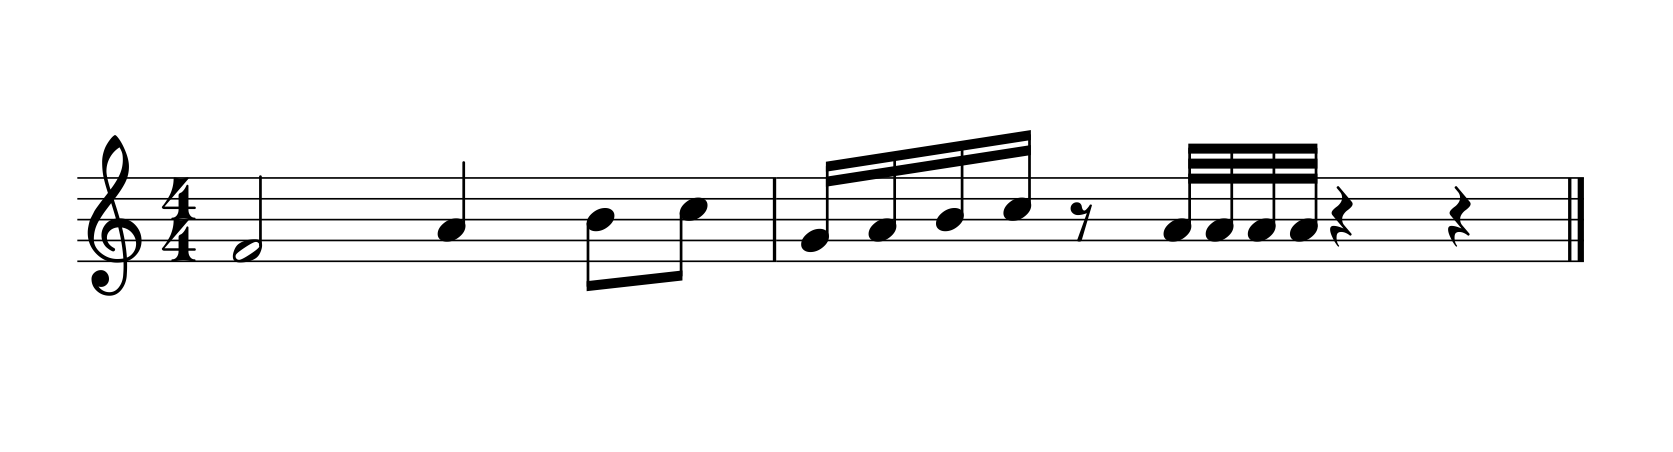
\includegraphics[width=150mm, keepaspectratio]{sheets/sheet01.png}
\caption{Egyszer� kotta f�l-, negyed-, nyolcad-, tizenhatod-, �s harmincketted hangokkal, valamint sz�netekkel} 
\label{fig:sheet01}
\end{figure} 

A kott�n a hangok p�rhuzamos vonalakon helyezkednek el, amelyek a hangmagass�gokat jel�lik. A zenei hangoknak gomb�cok felelnek meg, melyeket a latin �b�c� (C, D, E, F, G, A, H) bet�ir�l neveztek el. Ha egy hang m�lys�ge vagy magass�ga miatt nem f�r el az alap �t vonal valamelyik�n (vagy k�z�tt�k), a kotta p�tvonalakkal eg�sz�thet� ki.

A zene ritmus�t a hangok hossza hat�rozza meg. Az egys�ghossz� hangot �res, sz�rn�lk�li gomb�c jel�li, a f�lhangot �res gomb�c sz�rral, a negyedet (t�) teli gomb�c sz�rral. A negyedn�l kisebb hangok eset�n a hangokat �sszek�t� gerend�k sz�ma hat�rozza meg a hang hossz�s�g�t. Egy gerend�val vannak �sszek�tve a nyolcadok (ti), kett�vel a tizenhatodok, h�rommal a harminckettedek �s �gy tov�bb (L�sd: \ref{fig:sheet01}
�bra).

Az aktu�lisan jel�lt hang hossz�t m�sf�lszerezi a gomb�c melletti pont, �gy egy negyedb�l h�romnyolcad, nyolcadb�l h�romtizenhatod, stb\dots hossz�s�g� hangot k�pez. 

A kulcs ut�n �ll� k�t egym�s f�l�tt l�v� eg�sz sz�m azt jel�li, hogy az �temek h�ny azonos hossz�s�g� hangjegyet tartalmazhatnak. Az �temeket f�gg�leges vonal, az �temvonal v�lasztja el egym�st�l. Az ezek k�zti hangok (�s sz�netek) �sszhossz�s�ga azonos, �s megegyezik az �temjelz�sben megadott �rt�kkel (4/4 eset�n n�gy negyed hossz� �temek).

A triola egy olyan h�rom hangjegyb�l �ll� csoport, amely nem rendes �rt�kekre t�maszkodik. P�ld�ul ha szab�lyszer�leg egy negyed hangjegyre k�t nyolcad esne, triola eset�n a hangot h�rom ,,nyolcadra'' osztjuk. A kott�n ezt egy sz�m jel�li a hangokat �sszek�t� gerend�n. �t hangjegyb�l �ll� verzi�j�nak neve kvintola.

Ezeken k�v�l vannak tov�bbi m�dos�t�-, illetve felold�jelek, melyek r�szletez�s�be itt nem megyek bele.

%----------------------------------------------------------------------------
\section{A n�pzenekutat�s}
%----------------------------------------------------------------------------

A n�pzenekutat�s...

%----------------------------------------------------------------------------
\subsection{A zenei rendszerez�s}
%----------------------------------------------------------------------------

A n�pzene rendszerez�s�nek �tlete a finn kutat�t�l, Ilmari Krohnt�l sz�rmazik, aki a finn tudom�nyos n�pdalgy�jtem�ny rendez�s��rt �s szerkeszt�s��rt volt felel�s. Kod�ly Zolt�n �s Bart�k B�la is felhaszn�lta a t�le sz�rmaz� rendszerez�si elvet a magyar n�pzene katalogiz�l�sa sor�n.

%----------------------------------------------------------------------------
\subsection{A muzikol�gia}
%----------------------------------------------------------------------------

A muzikol�gia, vagy zeneelm�let az �ltal�nos �s magyar zenet�rt�net, historiogr�fia, zenei filol�gia, zenei szociol�gia, bibliogr�fia ter�let�vel foglalkoz� tudom�ny \cite{PortalDeb}. M�vel�i a magasabb szint� �sszhangzattani, formatani, ellenponttani ismeretek, st�lustanulm�nyok, zeneelm�let, zenet�rt�net, valamint kottaolvas�si k�szs�g ter�leteken rendelkeznek specializ�lt szaktud�ssal.

%----------------------------------------------------------------------------
\chapter{A ritmus}
%----------------------------------------------------------------------------

A ritmus g�r�g eredet� sz�, jelent�se: l�ktet�s, dobog�s, (sz�v-)ver�s, �tem. Hasonl� vagy azonos elemek id�beli szab�lyos v�ltakoz�s�t, ism�tl�d�s�t �rtj�k alatta. A zene csak az id�ben foghat� fel, teh�t nem �rtelmezhet� a ritmus fogalma n�lk�l.

A dallam �s a ritmus egy�ttesen hat�roznak meg egy dalt, azt azonban nem mondhatjuk, hogy egym�st�l elv�laszthatatlanok, hiszen gyakran ugyanazt a dallamot teljesen m�s ritmussal hallhatjuk, illetve a k�l�nb�z� eredet� �s tulajdons�g� dallamok el�fordulnak azonos ritmussal \cite{Vargyas1}. 

A n�pdalok rendszerez�s�ben a dallam �s a ritmus szerinti megk�zel�t�s mindig p�rhuzamosan �rv�nyes�lt.

%----------------------------------------------------------------------------
\section{A ritmusok �sszehasonl�t�sa}
%----------------------------------------------------------------------------

Mind adatb�ny�szati, mind zeneelm�leti szempontb�l alapvet� k�rd�s, hogy hogyan hasonl�tsunk �ssze k�t ritmust. A ritmusok reprezent�ci�j�t �gy kell megv�lasztanunk, hogy azok �sszehasonl�that�ak legyenek olyan m�don, amit a zenekutat� �rtelmesnek tal�l. Alapvet� k�vetelm�ny, hogy ez az �sszehasonl�t�s emberi �szlel�s�nkkel �sszhangban legyen, azaz hasonl�nak �rz�kelt ritmusokat hasonl�nak, k�l�nb�z�nek �rz�kelt ritmusokat pedig k�l�nb�z�nek tal�ljon.

K�t ritmus ($r_i$ �s $r_j$) k�l�nb�z�s�g�t valamik�pp m�rhet�v� kell tenn�nk. Meg kell adnunk egy formul�t ($d(r_i,r_j)$), amely a kapott k�t ritmus�br�zol�s alapj�n k�pes meghat�rozni egy k�l�nb�z�s�get t�kr�z� numerikus �rt�ket. K�zenfekv� megk�zel�t�snek t�nik, ha ezt a k�l�nb�z�s�gi �rt�ket a $0$ �s $1$ k�z�tti sk�l�n helyezz�k el, ahol min�l kisebb az �rt�k, ann�l jobban hasonl�t egym�sra a k�t ritmus. A $0$ jelenti a teljes ritmikai azonoss�got, m�g az $1$ a lehet� legnagyobb k�l�nb�z�s�get, a k�t sz�ls��rt�k k�z�tt pedig egyenesen ar�nyosan oszlik el a k�l�nb�z�s�g. 

Az �ltal�nos t�vols�gf�ggv�nnyel szemben t�masztott form�lis k�vetelm�nyek a k�vetkez�k:

\begin{enumerate}
\item $d(x,y) \geq 0, \forall x,y$-ra �s $d(x,y)=0 \Leftrightarrow x=y$, azaz k�t elem t�vols�ga nem negat�v, �s nulla akkor �s csak akkor, ha a k�t elem azonos.
\item $d(x,y) = d(y,x)$. Az $x$ �s az $y$ elem t�vols�ga mindk�t ir�nyban ugyanaz (szimmetria).
\item $d(x,z) \leq d(x,y) + d(y,z), \forall x,y,z$-re (h�romsz�g-egyenl�tlens�g).
\end{enumerate}

A szimmetria megk�vetel�se eset�nkben nem felt�tlen�l sz�ks�ges, ezt a feladat speci�lis jellemz�i �s a kiv�lasztott metrika saj�toss�gai hat�rozz�k meg.

%----------------------------------------------------------------------------
\section{A t�vols�gok t�rol�sa}
%----------------------------------------------------------------------------

Az alapelk�pzel�s szerint minden ritmus �sszehasonl�t�sra ker�l az �sszes t�bbi ritmussal, a kisz�m�tott �rt�kek pedig egy �gynevezett k�l�nb�z�s�gi m�trix ($M_{diff}$) megfelel� hely�re ker�lnek. Ezt �gy k�pezz�k, hogy vessz�k egy sorba az �sszes ritmust, illetve vessz�k �ket egy oszlopba is, majd a kapott t�bl�zat megfelel� hely�re be�rjuk a k�l�nb�z�s�gi �rt�ket. A m�trix f��tl�j�ban nyilv�nval�an csupa null�k �llnak, hiszen $r_i$ ritmus megegyezik $r_i$ ritmussal, azaz $d(r_i,r_i)=0, \forall i$-re (\ref{eq:form01} k�plet). Ebben az esetben $n*(n-1)$ �sszehasonl�t�st kell elv�gezn�nk �s ennyi eredm�nyt is kell t�rolnunk.

\begin{align}
\label{eq:form01}
M_{diff} = \bordermatrix{~ & r_1 & r_2 & r_3 & \cdots & r_{n-1} & r_n \cr
                  r_1 & 0 & d(r_1,r_2) & d(r_1,r_3) & \cdots & d(r_1,r_{n-1}) & d(r_1,r_n) \cr
									r_2 & d(r_2,r_1) & 0 & d(r_2,r_3) & \cdots & d(r_2,r_{n-1}) & d(r_2,r_n) \cr
									r_3 & d(r_3,r_1) & d(r_3,r_2) & 0 & \cdots & d(r_3,r_{n-1}) & d(r_3,r_n) \cr
									\vdots & \vdots & \vdots & \vdots & \ddots & \vdots & \vdots \cr
									r_{n-1} & d(r_{n-1},r_1) & d(r_{n-1},r_2) & d(r_{n-1},r_3) & \cdots & 0 & d(r_{n-1},r_n) \cr
                  r_n & d(r_n,r_1) & d(r_n,r_2) & d(r_n,r_3) & \cdots & d(r_n,r_{n-1}) & 0\cr}
\end{align}

Amennyiben �gy d�nt�nk, hogy a megk�vetelj�k t�vols�gf�ggv�ny szimmetri�j�t is, akkor a m�trix is szimmetrikus lesz (hiszen ekkor l�nyegtelen, hogy $r_i$ ritmust vetj�k �ssze $r_j$-vel, vagy $r_j$ ritmust $r_i$-val, azaz $d(r_i,r_j)=d(r_j,r_i), \forall i,j$-re). Ekkor a k�nnyebb t�rol�s �s feldolgoz�s �rdek�ben el�g, ha csak a f��tl� alatti elemeket tekintj�k.

\begin{align}
\label{eq:form02}
M_{diff} = \bordermatrix{~ & r_1 & r_2 & r_3 & \cdots & r_{n-1} & r_n \cr
                  r_1 & 0 & - & - & \cdots & - & -\cr
									r_2 & d(r_2,r_1) & 0 & - & \cdots & - & -\cr
									r_3 & d(r_3,r_1) & d(r_3,r_2) & 0 & \cdots & - & -\cr
									\vdots & \vdots & \vdots & \vdots & \ddots & \vdots & \vdots \cr
									r_{n-1} & d(r_{n-1},r_1) & d(r_{n-1},r_2) & d(r_{n-1},r_3) & \cdots & 0 & -\cr
                  r_n & d(r_n,r_1) & d(r_n,r_2) & d(r_n,r_3) & \cdots & d(r_n,r_{n-1}) & 0\cr}
\end{align}


A \ref{eq:form02} k�pletben szerepl� m�trix-defin�ci�ban l�that�, hogy szimmetria eset�n mely �rt�kekre nincs sz�ks�g�nk, melyek adottak �s melyeket kell kisz�molnunk. Adott $n$ sz�m� ritmust felt�telezve k�nny� meghat�rozni, hogy ehhez �sszesen $\frac{n^2-n}{2}$ �sszehasonl�t�s sz�ks�ges.

N�h�ny t�zezer elemb�l �ll� adatb�zis eset�n az �gy kapott $M_{diff}$ mem�ri�ban is t�rolhat�, ha azonban tov�bbn� az adathalmaz m�rete, megfontoland� a mem�ri�ban csak minden elem $k$ legk�zelebbi szomsz�dj�t�l val� t�vols�g�t t�rolni. A projekt jelenlegi f�zis�ban a kisebb m�ret miatt ezzel nem kell foglalkoznunk.

%----------------------------------------------------------------------------
\section{A ritmus geometriai reprezent�ci�ja}
%----------------------------------------------------------------------------

A ritmus vizu�lis megjelen�t�se nem csak k�nnyebb elemz�st tesz lehet�v�, de olyan tulajdons�gokra h�vhatja fel a figyelmet, melyek fontosak a hasonl�s�g m�r�s�hez. 

A $13$. sz�zadi arab zenetud�s, Safi al-Din �ta ismert a ritmus azon szeml�ltet�se, mely egy k�rt k�rcikkekre bont, az �t�sekhez tartoz� k�rcikkeket kisz�nezi, a sz�netekhez tartoz�kat pedig �resen hagyja \cite{Toussaint3}. A kezd�pontot egy ny�l jelzi. Ez a zseni�lisan egyszer� m�dszer a ritmus ciklikuss�g�t is megragadja, hiszen egy ritmus t�bb versszakb�l, str�f�b�l �ll� dalok eset�n visszat�r. 

\begin{figure}[!h]
\centering
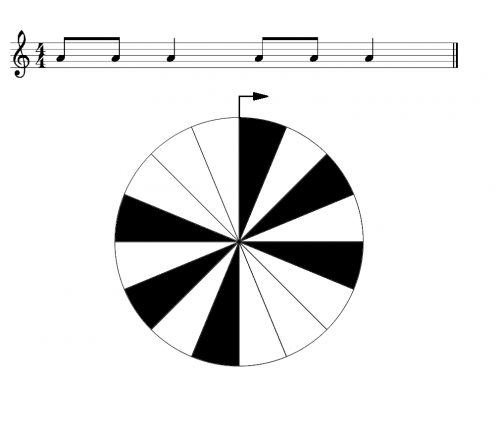
\includegraphics[width=100mm, keepaspectratio]{figures/chart01.png}
\caption{A ritmus 13. sz�zadb�l sz�rmaz� ciklikus �br�zol�sa} 
\label{fig:fig01}
\end{figure}

A \ref{fig:fig01} �br�n l�that� egy egyszer� ti-ti-t� ti-ti-t� ritmus �br�zol�sa. A teljes k�r $16$ egyenl� k�rcikkre van osztva, a hangs�lyos �temek elej�hez tartoz� k�rcikkek kit�lt�ttek, az ut�nuk k�vetkez�, az �tem hossz�s�g�t�l f�gg� sz�m� k�rcikkek pedig kit�ltetlenek. R�videbb �temek (pl. tizenhatodok) szeml�letes �br�zol�s�hoz nagyobb felbont�s� k�r�ket kell alkalmaznunk. Az �bra tengelyes vagy k�z�ppontos szimmetri�ja fontos inform�ci�t hordoz a megjelen�tett ritmusr�l is.


\begin{figure}[!h]
\centering
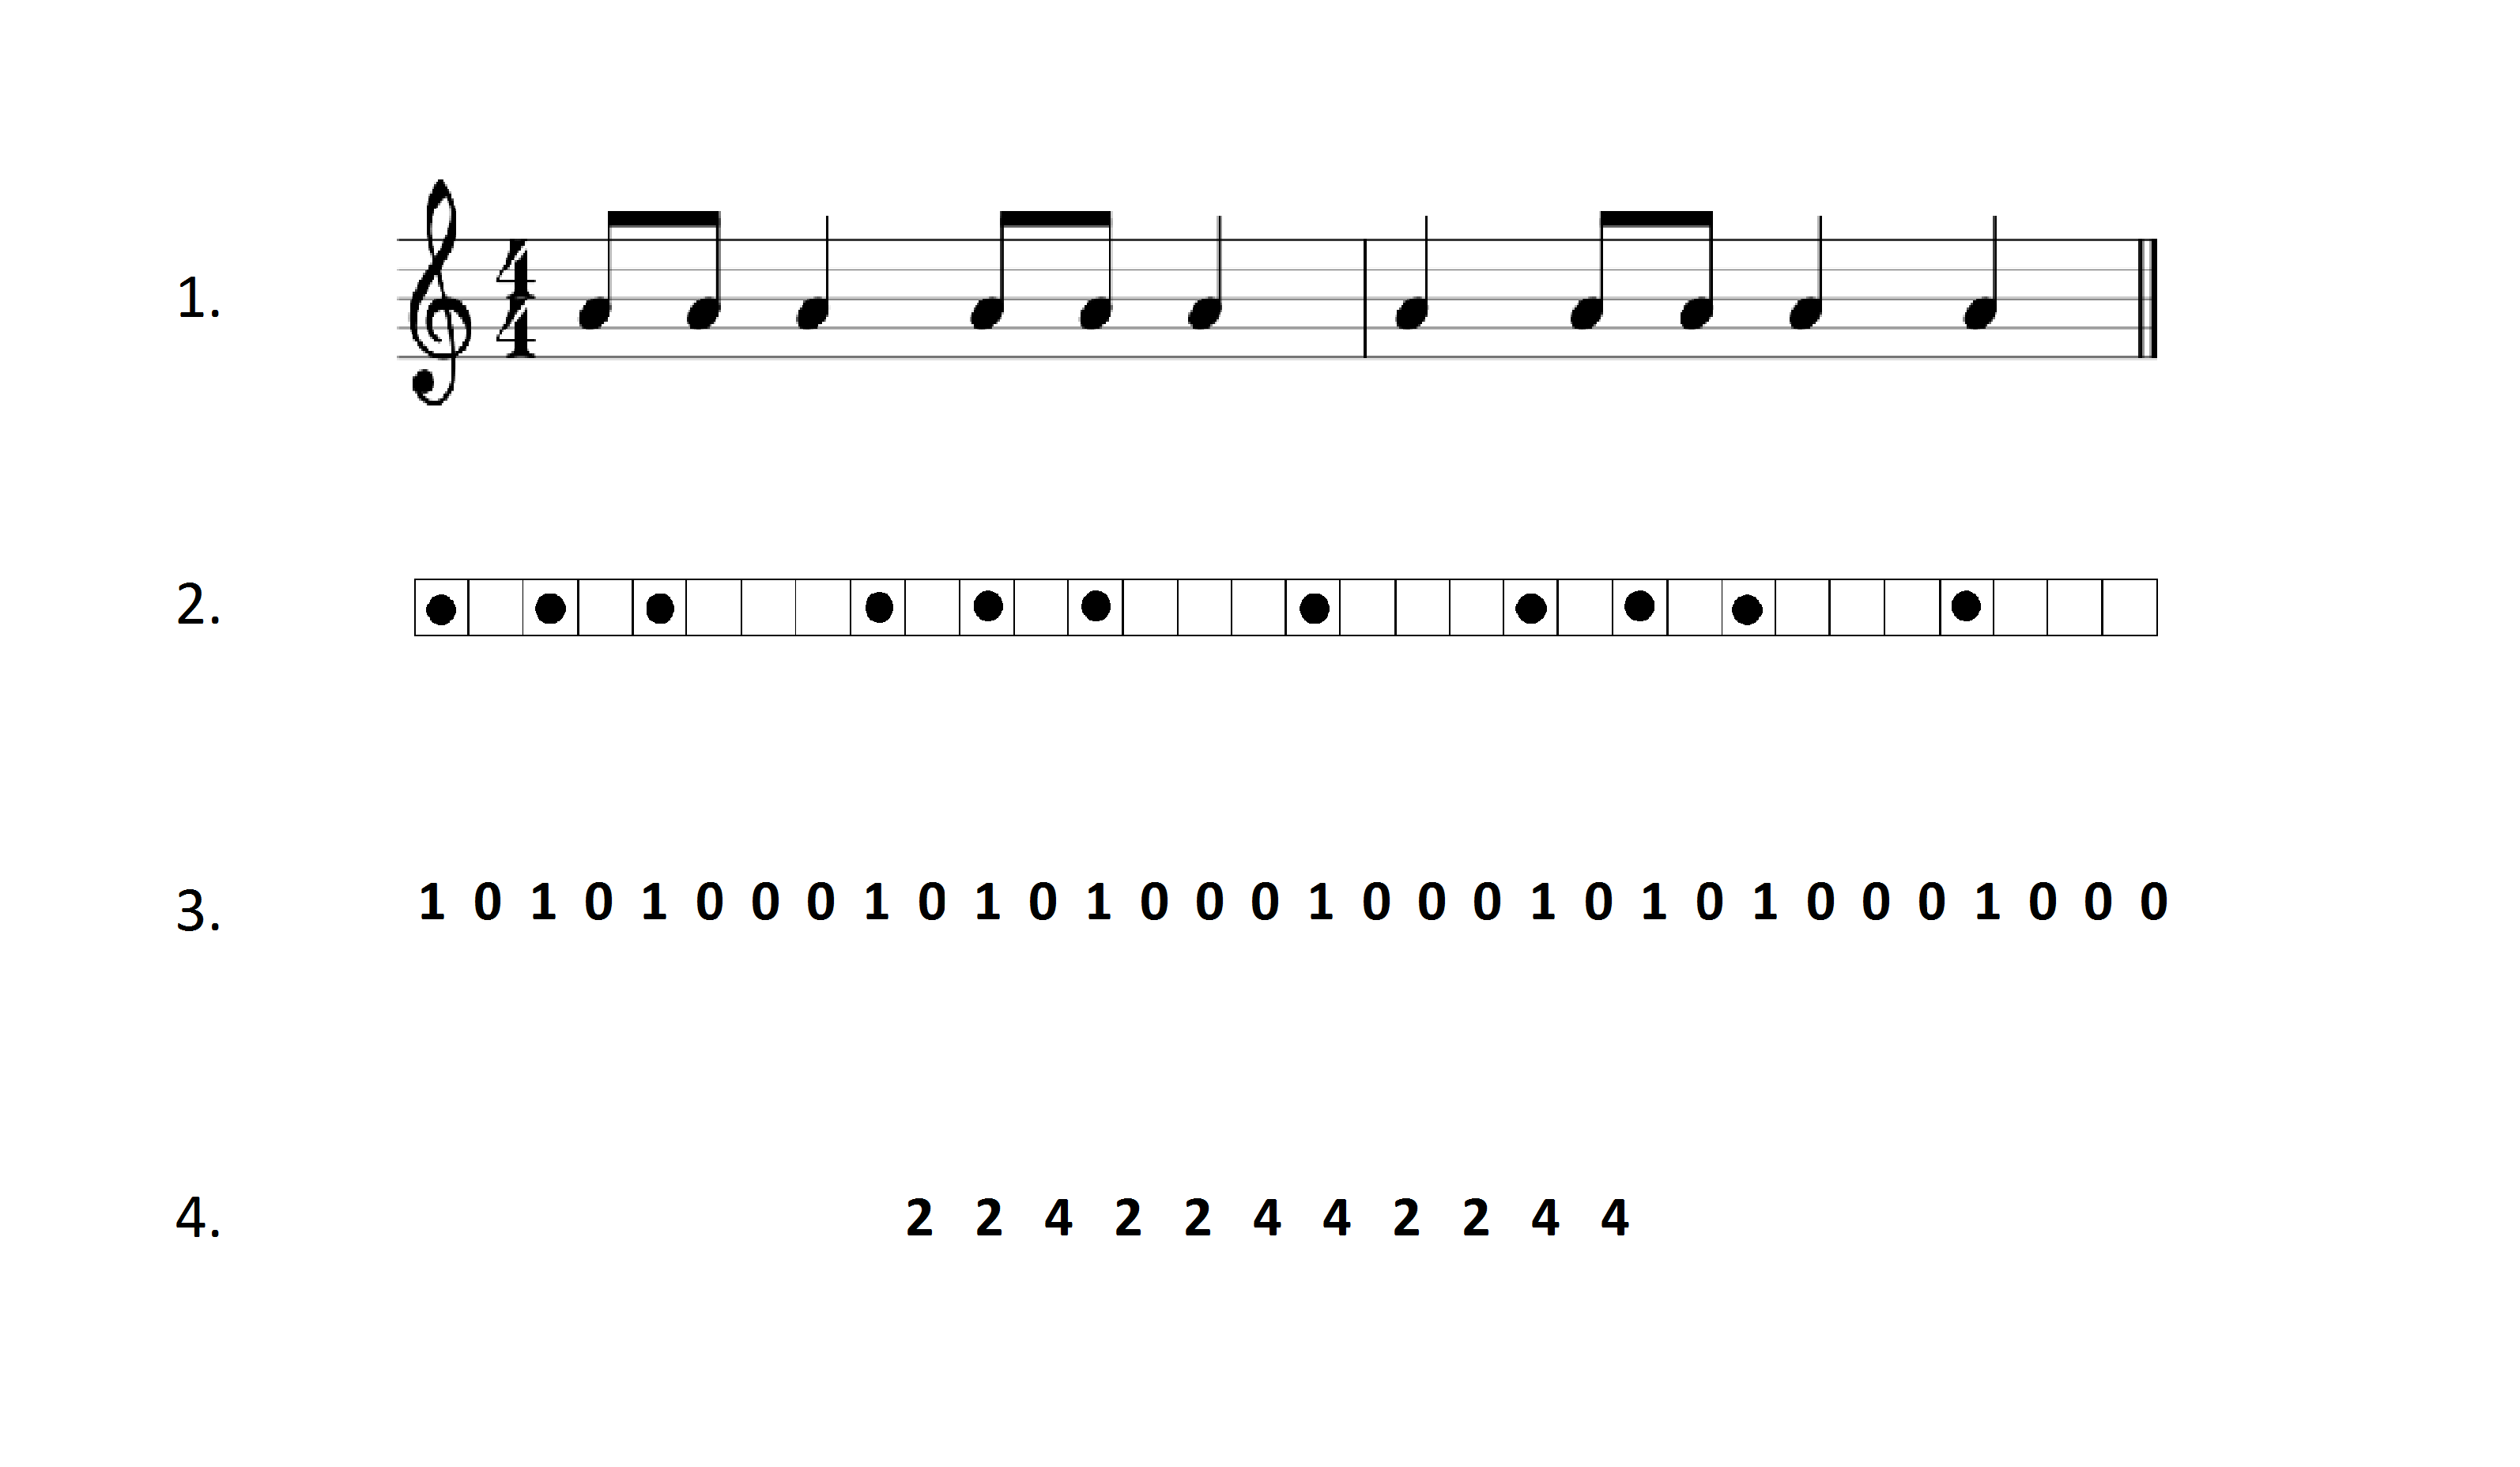
\includegraphics[width=150mm, keepaspectratio]{figures/ritmus.png}
\caption{N�gy k�l�nb�z� ritmus�br�zol�s} 
\label{fig:fig02}
\end{figure}

%----------------------------------------------------------------------------
\subsection{Time Unit Box System}
%----------------------------------------------------------------------------

A ritmusok g�pi �br�zol�s�ra a University of California (UCLA) kutat�i �ltal kifejlesztett Time Unit Box System (TUBS) m�dszer t�nik a legalkalmasabbnak (a \ref{fig:fig02} �br�n a 2. m�dszer). Ez n�h�ny egym�s mell� helyezett dobozb�l �ll, melyek mindegyike egy el�re meghat�rozott id�szeletet reprezent�l. A dobozok vagy �resek, vagy jel�ltek lehetnek, az �res doboz a hozz� tartoz� id�szeletben zenei esem�ny hi�ny�t, m�g a jel�lt doboz a annak megl�t�t t�kr�zi. Ez a megk�zel�t�s k�nnyed�n interpret�lhat� a sz�m�t�studom�ny �ltal egyszer�en feldolgozhat� bin�ris vektor nyelv�n is (a \ref{fig:fig02} �br�n a 3. m�dszer).

\begin{figure}[!h]
\centering
	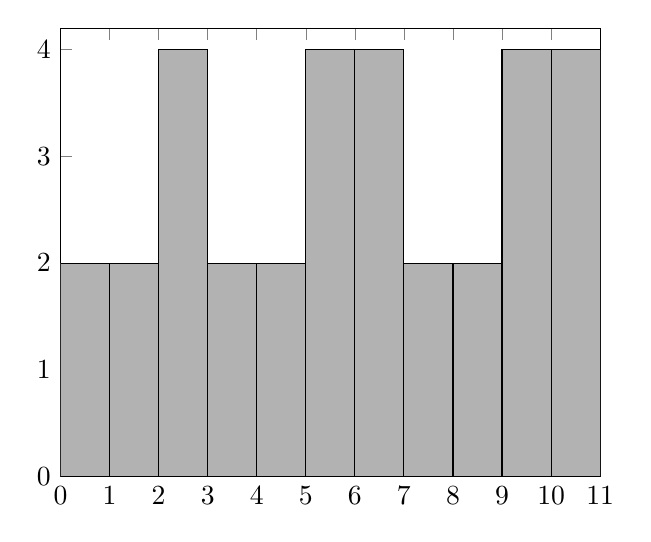
\begin{tikzpicture}
	\begin{axis}[ymin=0,ymax=4.2,enlargelimits=false,xtick=data]
	\addplot
	[ybar interval,fill=black!30]
	coordinates
	{(0, 2) (1,    2) (2,    4) (3,    2) (4,    2) (5,    4) (6,    4)
	 (7, 2) (8, 2) (9, 4) (10, 4) (11, 4)};
	\end{axis}
	\end{tikzpicture}
\caption{Szomsz�dos intervallumok spektruma}
\label{fig:fig03}
\end{figure}

Megjegyzend�, hogy triol�k, illetve egy�b nem szab�lyos �rt�kekre t�maszkod� ritmikai elemek reprezent�l�s�ra ez a m�dszer csak jelent�s felbont�s n�veked�ssel alkalmas. A felbont�s pontos m�rt�ke f�gg az el�fordul� szab�lytalan elemek t�pusait�l is.

%----------------------------------------------------------------------------
\subsection{Szomsz�dos intervallumok �br�zol�sa}
%----------------------------------------------------------------------------

A \ref{fig:fig02} �br�n l�that� $4$. ritmus�br�zol�si m�dszerben tal�lhat� sz�mok azt jelzik, hogy milyen hossz�ak az egym�st k�vet� hangs�lyos elemek. A ti-ti-t� ritmus �gy tizenhatodos felbont�ssal a
\[ \left( \begin{array}{ccc}
2& 2& 4
\end{array} \right)
\]
intervallum-vektorral jellemezhet�. 

Ennek a vektornak a szeml�ltet�s�re a University of Oxford kutat�i dolgoztak ki m�dszereket. Ezek egyike, a szomsz�dos intervallumok spektrum�nak m�dszere �gy �br�zolja a ritmust egy koordin�ta-rendszerben, hogy az $x$ tengely ment�n egyes�vel haladva egy-egy oszlop magass�ga felel meg az adott poz�ci�ban �ll� hangs�ly hossz�nak (\ref{fig:fig03} �bra). Az azonos �temet tartalmaz� ritmusok �gy szeml�letesen �br�zolhat�ak egym�s mellett vagy alatt, de ez a m�dszer megnehez�ti az intervallumok relat�v hossz�s�g�nak �rz�kel�s�t.

\begin{figure}[!h]
\centering
	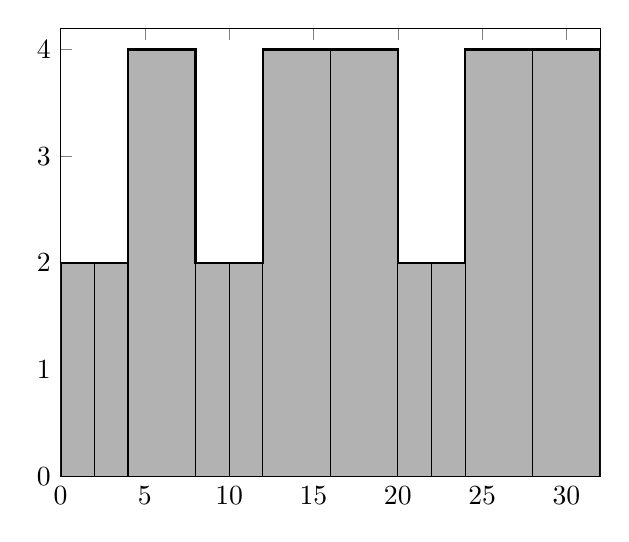
\begin{tikzpicture}
	\begin{axis}[ymin=0,ymax=4.2,enlargelimits=false]
	\addplot
	[ybar interval,fill=black!30]
	coordinates
	{(0, 2) (2,    2) (4,    4) (8,    2) (10,    2) (12,    4) (16,    4)
	 (20, 2) (22, 2) (24, 4) (28, 4) (32, 4)};
	\addplot
	[const plot,thick]
	coordinates
	{(0, 0) (0, 2) (2,    2) (4,    4) (8,    2) (10,    2) (12,    4) (16,    4)
	 (20, 2) (22, 2) (24, 4) (28, 4) (32, 4) (32, 0)};
	\end{axis}
	\end{tikzpicture}
\caption{Temporal Elements Displayed As Squares (TEDAS)}
\label{fig:fig04}
\end{figure}

K�zenfekv� �tlet a h�tr�nyok kik�sz�b�l�s�re a k�l�nb�z� m�dszerek �tv�zete. A TUBS m�dszert �s a szomsz�dos intervallumok spektrum�nak m�dszer�t �gy tudjuk vegy�teni, hogy minden TUBS-ban szerepl� dobozba azt a sz�mot �rjuk, amilyen hossz� a hozz� tartoz� vagy az �t megel�z� hangs�lyos elem. Ha az �gy kapott vektort �br�zoljuk a koordin�ta-rendszerben, akkor egy olyan �br�t kapunk, melyen az id�beli elemek megfelel� m�ret� n�gysz�gekkel vannak reprezent�lva. Ebb�l sz�rmazik a m�dszer elnevez�se is: Temporal Elements Displayed As Squares, vagy r�viden TEDAS \cite{Toussaint2}. 

A kor�bbiakban t�rgyalt ritmushoz tartoz� TEDAS �br�zol�s l�that� a \ref{fig:fig04} �br�n. Az alapj�ul szolg�l� vektort, melyet kronotonikus l�ncnak nevez�nk, nem csak oszlopk�nt, hanem f�ggv�nyk�nt is �br�zolhatjuk a koordin�ta-rendszerben (\ref{fig:fig05} �bra).


\begin{figure}[!h]
\centering
        \begin{subfigure}[b]{0.5\textwidth}
                \centering
               
\includegraphics[width=80mm, keepaspectratio]{figures/ritmusok.png}
                \caption{Ritmusok}
        \end{subfigure}%
        \begin{subfigure}[b]{0.5\textwidth}
                \centering
								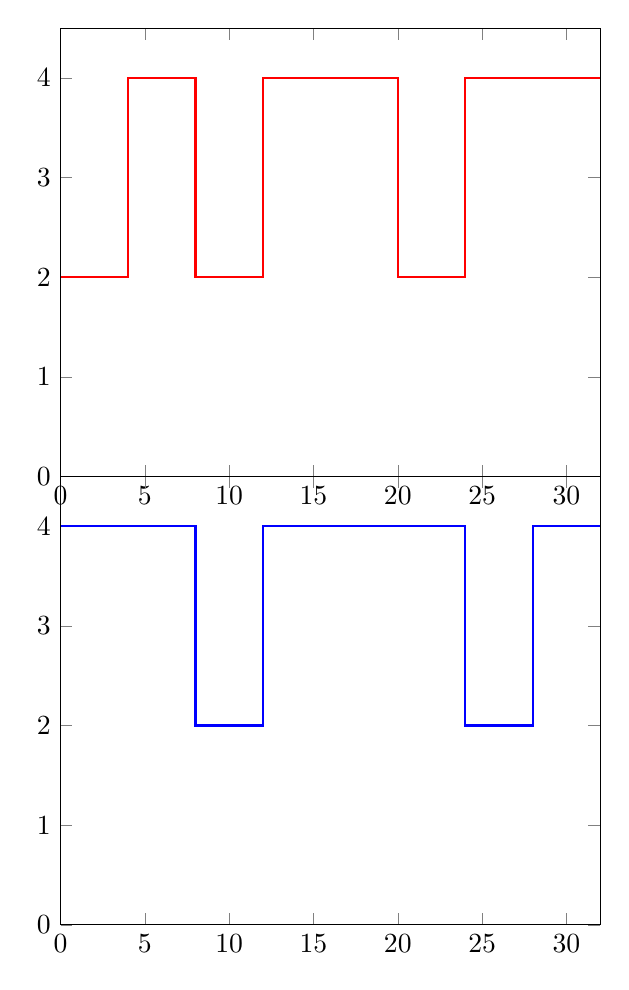
\begin{tikzpicture}
									\begin{groupplot}[
											group style={
													group name=my plots,
													group size=1 by 2,
													xlabels at=edge bottom,
													vertical sep=0pt
											},
											xmin=0, xmax=32,
											ymin=0, ymax=4.5
									]
									\nextgroupplot
									\addplot[const plot,red, thick] coordinates
									{(0,    2) (4,    4) (8,    2) (12,    4) (20,    2) (24,    4) (28,    4) (32,    4)};
									\nextgroupplot
									 \addplot [const plot, blue, thick] coordinates
									{(0,    4) (8,    2) (12,    4) (24,    2) (28,    4) (32,    4)};
									\end{groupplot}
								\end{tikzpicture}
                \caption{Kronotonikus l�ncok}
        \end{subfigure}
\caption{Kronotonikus l�ncok �rtelmez�se}
\label{fig:fig05}
\end{figure}


%----------------------------------------------------------------------------
\section{Ritmikus k�l�nb�z�s�gi metrik�k}
%----------------------------------------------------------------------------

A mindennapi �letben hossz�s�gk�nt �rtelmezett t�vols�g fogalm�t a matematika �ltal�nos�tja �s k�l�nb�z� m�dokon defini�lt m�rt�keket, metrik�kat vezet be. A ritmus-reprezent�ci�kat akkor tudjuk �sszehasonl�that�v� tenni, ha a k�zt�k l�v� t�vols�got egy nemnegat�v skal�rmennyis�ggel jel�lj�k. Az irodalom b�s�gesen foglalkozik a t�m�val, az �ltalam v�lasztott m�dszerek nagyobbik r�sze Godfried Toussaint \cite{Toussaint1}, illetve Lior Rokach \cite{Rokach} cikkeib�l sz�rmazik, de gyakran tov�bbi pontos�t�sra �s kieg�sz�t�sre szolg�ltak az �ltaluk v�zolt �ltal�nosabb elj�r�sok.

%----------------------------------------------------------------------------
\subsection{Hamming-t�vols�g}
%----------------------------------------------------------------------------
A sz�m�t�studom�nyban bin�ris vektorok �sszehasonl�t�s�nak legterm�szetesebb m�dja a vektorok elemenk�nti �sszehasonl�t�sa, ismertebb nev�n Hamming-t�vols�g sz�mol�sa. Ebben a megk�zel�t�sben a TUBS m�don reprezent�lt ritmusok k�zvetlen�l haszn�lhat�k, hiszen azok l�nyeg�ben bin�ris vektorok. A m�dszer elm�leti h�tter�ben az $n$ hossz� vektorok egy $n$-dimenzi�s hiperkocka pontjai. Adott $X=(x_1,x_2,...,x_n)$ �s $Y=(y_1,y_2,...,y_n)$ k�z�tti t�vols�g sz�molhat� az al�bbi k�plet seg�ts�g�vel:
\begin{align}
d_H(X,Y)=\sum_{i=1}^n |x_i-y_i|
\end{align}
ahol $|x|$ az $x$ �rt�k abszol�t �rt�k�t jel�li.

A m�dszer nagyon egyszer�, id�ig�nye is alacsony, hiszen el�g egyetlen ciklusban v�gigiter�lni a vektorokon �s akkumul�lni a k�l�nb�z� bitek sz�m�t, azaz l�p�ssz�ma a vektor hossz�nak konstans-szorosa ($O(n)$). Ugyanakkor nem biztos, hogy  erre a speci�lis ig�nyre a legjobban megfelel, mert az k�l�nb�z�s�get ugyan j�l m�ri, de azt nem, hogy milyen messze vannak egym�st�l az elt�r�sek. A gyakorlati tapasztalatok azt mutatj�k, hogy egy hangs�ly t�volabbra helyez�se k�l�nb�z�bbnek hat, mintha k�zelebbre tett�k volna �t. Szint�n h�tr�nya a m�dszernek, hogy egy �temmel eltolva ugyanaz a ritmus teljesen m�snak �rt�kel�dik, holott az emberi f�l sz�m�ra az nagyon hasonl� az eredetihez.

%----------------------------------------------------------------------------
\subsection{Bin�ris vektorok t�vols�ga}
%----------------------------------------------------------------------------

Az irodalom \cite{Rokach} �ltal javasolt �ltal�nos m�dszer bin�ris vektorok �sszehasonl�t�s�ra k�t esetet k�l�nb�ztet meg. Abban az esetben, ha a bin�ris vektorban a $0$ illetve az $1$ �rt�k azonos val�sz�n�s�ggel fordul el�, szimmetrikus attrib�tumr�l besz�l�nk �s a k�vetkez�k�pp hat�rozhatjuk meg az $X$ �s $Y$ bin�ris vektorok k�z�tti t�vols�got:
\begin{align}
d_{Bin1}(X,Y)=\frac{r+s}{q+r+s+t} 
\end{align}

ahol $q$ az azonos helyen l�v� $1$-esek, $t$ az azonos helyen l�v� $0$-�k, $s$ �s $r$ pedig a k�l�nb�z� bitek sz�ma $X$-ben, illetve $Y$-ban (ha azonos hossz�ak, akkor $s=r$). Ez egyfajta s�lyozott Hamming-t�vols�gk�nt is �rtelmezhet�.

A kor�bbiakkal szemben aszimmetrikus attrib�tumr�l akkor besz�l�nk, ha a $0$ �s $1$ k�l�nb�z� val�sz�n�s�ggel fordul el� a vektorokban, �gy teh�t az egyik�k egyez�se ,,fontosabb'', mint a m�sik� (�ltal�ban ez az $1$-esek egyez�se). Ekkor a nevez�b�l elhagyjuk a null�k egyez�s�t sz�ml�l� $t$-t:
\begin{align}
d_{Bin2}(X,Y)=\frac{r+s}{q+r+s} 
\end{align}

A ritmusokat reprezent�l� TUBS vektorok �ltal�nos jellemz�je, hogy t�bb benn�k a sz�net, mint a hangs�lyos elem (az $1$-es), ez�rt a m�sodikk�nt defini�lt megk�zel�t�st haszn�ljuk ink�bb.

Ez a megk�zel�t�s sajnos szint�n rendelkezik a Hamming-t�vols�g minden, kor�bban v�zolt h�tr�ny�val.

%----------------------------------------------------------------------------
\subsection{Intervallum-vektorok Manhattan-t�vols�ga}
%----------------------------------------------------------------------------

Zenefelismer� �s zenekategoriz�l� algoritmusok �ltal gyakrabban haszn�lt ritmus�br�zol�s a hangs�lyok k�z�tti intervallumok hosszait reprezent�l� vektorokon alapul (a \ref{fig:fig02} �br�n a 4. m�dszer hasonl�, de ott a hangs�lyos �temet is belesz�moljuk a hosszba, ez�rt ott a vektor minden eleme eggyel nagyobb). Egy ritmus az $X=(x_1,x_2,...,x_n)$ vektor �ltal reprezent�lt, ahol $x_1$ jel�li az els� hangs�ly ut�ni intervallum hossz�t. Az $X=(x_1,x_2,...,x_n)$ �s $Y=(y_1,y_2,...,y_n)$ �ltal jel�lt ritmusok k�z�tti Manhattan-t�vols�got az al�bbi formula adja meg:
\begin{align}
d_M(X,Y)=\sum_{i=1}^n |x_i-y_i| 
\end{align}
Az el�z� m�dszert�l mind�ssze annyiban t�r el, hogy egy m�s m�don k�pzett vektort vesz kiindul�si alapul, melynek elemei nem csak a $\left\{0,1\right\}$ halmazb�l ker�lhetnek ki. Az intervallum-vektorok $O(n)$ id�ben sz�molhat�k a TUBS �br�zol�sb�l, ebb�l k�vetkez�en a l�p�ssz�mban nincs elt�r�s ($O(n)$). Ez a megk�zel�t�s �gy �rtelmezhet� a mindennapi t�vols�ghoz k�pest, hogy egy olyan �t hossz�t m�ri, mely egym�sra mer�leges szakaszokon haladva vezet az egyik pontb�l a m�sikba, mintha csak egy nagyv�rosi �th�l�zaton haladhatn�nk.

%----------------------------------------------------------------------------
\subsection{Intervallum-vektorok Euklideszi-t�vols�ga}
%----------------------------------------------------------------------------

Az el�z� m�dszert tov�bbgondolva k�nnyen eljuthatunk a mindennapi �rtelemben vett t�vols�ghoz legk�zenfekv�bben illeszked� m�dszerhez, az Euklideszi-t�vols�ghoz. Egy, k�t, illetve h�rom dimenzi�ban pontosan azt is adja eredm�ny�l, mint amit egy vonalz�val m�rve kapn�nk. Egy ritmus ugyanaz az $X=(x_1,x_2,...,x_n)$ vektor �ltal reprezent�lt, ahol $x_1$ jel�li az els� hangs�ly ut�ni intervallum hossz�t. Az $X=(x_1,x_2,...,x_n)$ �s $Y=(y_1,y_2,...,y_n)$ �ltal jel�lt ritmusok k�z�tti Euklideszi t�vols�got �gy adhatjuk meg:
\begin{align}
d_E(X,Y)=\sqrt{\sum_{i=1}^n (x_i-y_i)^2} 
\end{align}

A kor�bbiakhoz hasonl�an ez az algoritmus is $O(n)$ l�p�st ig�nyel.

Az ut�bbi k�t megk�zel�t�s a Hamming-t�vols�gn�l alkalmasabb a ritmus k�l�nb�z�s�g�nek meghat�roz�s�hoz, hiszen az eltol�si probl�m�t kik�sz�b�lik.

%----------------------------------------------------------------------------
\subsection{Az intervallum-k�l�nb�z�s�gi vektorok t�vols�ga}
%----------------------------------------------------------------------------

Ez a m�dszer Coyle-t�l �s Shmulevich-t�l sz�rmazik. Az el�z�ekhez hasonl�an ez a megk�zel�t�s is az intervallum-vektorokb�l indul ki, �m miel�tt a k�t ritmus intervallumhosszait egym�shoz hasonl�tan�, az azonos ritmusban szomsz�dos elemekhez m�ri �ket. �gy egy ritmus az egym�st k�vet� intervallumok ar�nyival van jellemezve. Form�lisan a $T=(t_1,t_2,...,t_n)$ intervallum-vektor �ltal jel�lt ritmushoz egy olyan $X=(x_1,x_2,...,x_n)$ vektort defini�l, melynek elemei $x_i=t_{i+1}/t_i$ m�don vannak meghat�rozva. A ciklikuss�got is figyelembe v�ve $x_n=t_1/t_n$, �gy $T$-hez hasonl�an $X$ dimenzi�ja is $n$ lesz. Az �gy kapott $X$ vektort intervallum-k�l�nb�z�s�gi vektornak nevezz�k. Az $X=(x_1,x_2,...,x_n)$ �s $Y=(y_1,y_2,...,y_n)$ intervallum-k�l�nb�z�s�gi vektorok �ltal jel�lt ritmusok k�z�tti t�vols�got �gy defini�ljuk:
\begin{align}
d_{ID}(X,Y)=\big(\sum_{i=1}^n \frac{max(x_i,y_i)}{min(x_i,y_i)}\big)-n 
\end{align}

A szumm�zand� h�nyados �rt�ke mindig legal�bb $1$, ez�rt kell levonnunk bel�le a v�g�n $n$-t, hiszen annak nincs inform�ci�tartalma. Az algoritmus a kor�bbiakhoz hasonl�an $O(n)$ id�ben fut.

%----------------------------------------------------------------------------
\subsection{Cser�l�si t�vols�g}
%----------------------------------------------------------------------------

A negyedik, kor�bbiakt�l teljesen elt�r� megk�zel�t�s nem a k�l�nb�z�s�geket keresi, hanem azt sz�molja ki, hogy mennyi munka sz�ks�ges az egyik vektort a m�sikba transzform�lni. A genetik�ban sz�les k�rben haszn�lt m�dszer molekul�k egym�sba alak�t�s�hoz sz�ks�ges alapl�p�sek sz�m�t hat�rozza meg, ahol az alapl�p�sek valamilyen evol�ci�s mut�ci�t szimul�lnak.
Nek�nk egyszer�bb dolgunk van, az alapl�p�s ugyanis a pofonegyszer� csere m�velete. Annyit azonban meg kell k�tn�nk, hogy csak szomsz�dos elemeket cser�lhet�nk ki egym�ssal. 
\[ \left( \begin{array}{cccccccccccc}
1& 0& 1& 0& 1& 1& 0& 1& 0& 1& 0& 1
\end{array} \right)
\]
P�ld�ul a fenti ritmusvektor $4$ l�p�sben alak�that� �t a 
\[ \left( \begin{array}{ccccccccccccc}
1& 0& 1& 1& 0& 1& 1& 0& 1& 0& 1& 0
\end{array} \right)
\]
vektorr�, m�gpedig a harmadik, az �t�dik �s a hetedik hangs�lyos elem �s az azt megel�z� hangs�lytalan elem cser�j�vel. 

A cser�l�si t�vols�g kisz�m�t�s�hoz azonban nincs sz�ks�g�nk a t�nyleges cser�k v�grehajt�s�ra, hiszen az bizonyos esetekben nagyon k�lts�ges lenne. Ilyen p�ld�ul az al�bbi k�t ritmusvektor: 
\[ \left( \begin{array}{ccccccccccccc}
1& 1& 1& 1& 1& 1& 0& 0& 0& 0& 0& 0\\
0& 0& 0& 0& 0& 0& 1& 1& 1& 1& 1& 1
\end{array} \right)
\]
ahol a ritmus hossz�nak n�gyzet�vel ar�nyos csere sz�ks�ges. Ehelyett egy sokkal eleg�nsabb megold�st mutatunk. El�bb elt�roljuk azokat a poz�ci�kat, ahol hangs�lyos elem van. A fejezet els� p�ld�ira ez $U=(u_1,u_2,...,u_n) = (1,3,5,6,8,10,12)$ �s $V=(v_1,v_2,...,v_n) = (1,3,4,6,7,9,11)$. Az $u_i$ �s $v_i$ �rt�kek k�l�nbs�ge hat�rozza meg, hogy mennyi csere sz�ks�ges mindenk�ppen ahhoz, hogy a k�t �rt�khez tartoz� hangs�lyos elem a megfelel� helyen legyen. �ltal�noss�gban teh�t a cser�l�si t�vols�g a k�vetkez�k�pp sz�m�that� a fenti $U$ �s $V$ vektorok alapj�n:
\begin{align}
d_{SWAP}(X,Y)=\sum_{i=1}^n |u_i-v_i|
\end{align}

Az $U$ �s $V$ vektorok sz�mol�sa TUBS vektorokb�l $O(n)$ idej�, �gy $d(U,V)$ meghat�roz�s�hoz sem kell t�bb id�.

%----------------------------------------------------------------------------
\subsection{Kronotonikus t�vols�g}
%----------------------------------------------------------------------------

A Hofmann-Engl �ltal javasolt m�dszer a k�z�s koordin�ta-rendszerben �br�zolt kronotonikus l�ncokb�l indul ki. K�t ritmus t�vols�g�t �gy hat�rozza meg, hogy az �ltaluk meghat�rozott kronotonikus l�ncok alatti ter�leteket hasonl�tja �ssze. Form�lisan teh�t el�bb vessz�k az $f_1(x)$ �s $f_2(x)$ f�ggv�nyekkel le�rt kronotonikus l�ncok k�l�nbs�g�nek abszol�t �rt�k�t (amire az�rt van sz�ks�g, hogy ne null�zhassa ki k�t azonos m�ret� elt�r�s egym�st), majd ennek integr�lj�t (azaz a f�ggv�ny alatti ter�let nagys�g�t) tekintj�k a t�vols�gnak.
\begin{align}
d_K(X,Y) = K = \int |f_1(x)-f_2(x)|dx 
\end{align}
A \ref{fig:fig06} �bra szeml�lteti a kor�bbiakb�l m�r ismert ritmusokhoz tartoz� kronotonikus l�ncok k�z�tti kronotonikus t�vols�got.


\begin{figure}[!h]
\centering
	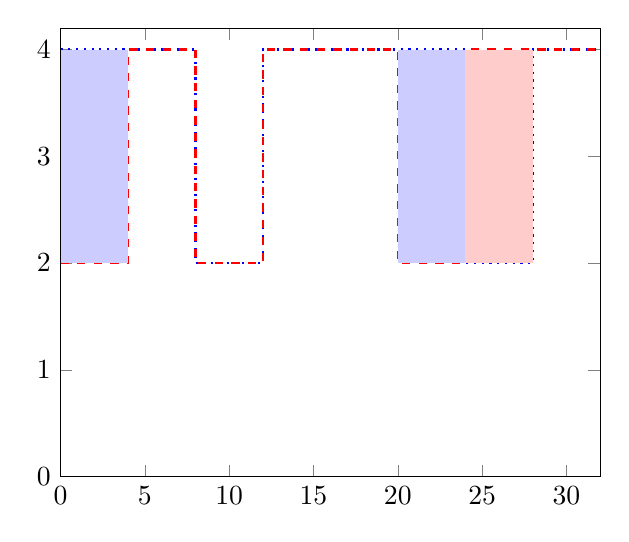
\begin{tikzpicture}
	\begin{axis}[ymin=0,ymax=4.2,enlargelimits=false]
	\addplot
	[const plot,blue, thick,dotted]
	coordinates
	{(0,    4) (8,    2) (12,    4) (24,    2) (28,    4) (32,    4)};
	\addplot
	[const plot, red, thick,style=dashed]
	coordinates
	{(0,    2) (4,    4) (8,    2) (12,    4) (20,    2) (24,    4) (28,    4) (32,    4)};
	\fill [blue,fill=blue!20] (axis cs:0,2) rectangle (axis cs:4,4);
	\fill [blue,fill=blue!20] (axis cs:20,2) rectangle (axis cs:24,4);
	\fill [red,fill=red!20] (axis cs:24,2) rectangle (axis cs:28,4);
	\end{axis}
	\end{tikzpicture}
\caption{K�t ritmus k�z�tti kronotonikus t�vols�g}
\label{fig:fig06}
\end{figure}

%----------------------------------------------------------------------------
\section{K�l�nb�z� hossz�s�g� ritmusok}
%----------------------------------------------------------------------------

A gyakorlatban a legritk�bb esetben fordul el�, hogy minden vizsg�lt ritmus hossza azonos. Az eddig t�rgyalt m�dszerek azonban egyt�l egyig felt�telezt�k ezt. Valamik�ppen teh�t m�dos�tanunk kell a kiindul�si algoritmusokon, hogy figyelembe vegy�k a ritmushosszok k�l�nb�z�s�g�t. 

Ugyanakkor ez a probl�ma ism�t felveti azt a k�rd�st is, hogy a defini�lt t�vols�gt�l megk�vetelj�k-e a szimmetri�t, azaz $d(x,y)$ �s $d(y,x)$ legyen-e egyenl� $\forall x,y$-ra, hiszen k�l�nb�z� hossz�s�g eset�n nem mindegy, hogy milyen sorrendben hajtunk v�gre bizonyos l�p�seket.

%----------------------------------------------------------------------------
\subsubsection{Szimmetria teljes�l�se eset�n}
%----------------------------------------------------------------------------

El�bb vizsg�ljuk meg azt az esetet, amikor teljes�l a szimmetria. Ez esetben k�zenfekv� megk�zel�t�s, ha a hosszabb ritmusvektort fixen hagyva tologatjuk (,,shiftelj�k'') a r�videbb vektort a hosszabb elej�t�l a v�g�ig, minden lehets�ges m�don sz�m�tunk egy t�vols�got, majd a kapott �rt�kek minimum�t vessz�k. 

Form�lisan teh�t, ha $|X|=n_1$, $|Y|=n_2$ �s $n_1>n_2$,  akkor 
\begin{align}
d_{Shifted}(X,Y) = \min_{i \in 0..n_1-n_2} d_{Spec}(X_{i,n_2+i},Y) 
\end{align}
ahol $X_{i,n_2+i}$ jel�li $X$ vektor $i.$ �s $n_2+i$. k�z�tti elemei �ltal alkotott vektort, bele�rtve a hat�rokat is. Az ily m�don meghat�rozott vektorok hossza m�r azonos, �gy �tadhat�k a kor�bbi szakaszban defini�lt elj�r�soknak ($d_{Spec} \in \left\{d_H,d_M,d_E,d_{ID},d_{SWAP}\right\}$). 

Ez a m�dszer szinkronban van azzal a gyakorlati megfigyel�ssel, hogy ha egy ritmus valahol mag�ban foglal egy m�sikat, akkor szoros kapcsolat van k�z�tt�k. A megk�zel�t�s h�tr�nya azonban, hogy nagy k�l�nbs�gek eset�n jelent�sen megn�velheti a fut�sid�t ($\forall i \in \left\{0,n_1-n_2\right\}$-re le kell futtatni az eredeti algoritmust). 

A g�rbe alatti ter�letekkel sz�mol� kronotonikus t�vols�g alap� algoritmusn�l enn�l egy szofisztik�ltabb megk�zel�t�st alkalmazhatunk. A m�dszer l�nyege, hogy a ritmusvektorokhoz rendelt kronotonikus vektorokat egy adott hossz�s�g� $x$-tengelyre vet�tj�k, f�ggetlen�l azok t�nyleges hossz�t�l. A k�l�nbs�gek meghat�roz�sa �s az integr�lsz�m�t�s az �gy kapott f�ggv�nyen t�rt�nik.

\begin{figure}[!h]
\centering
	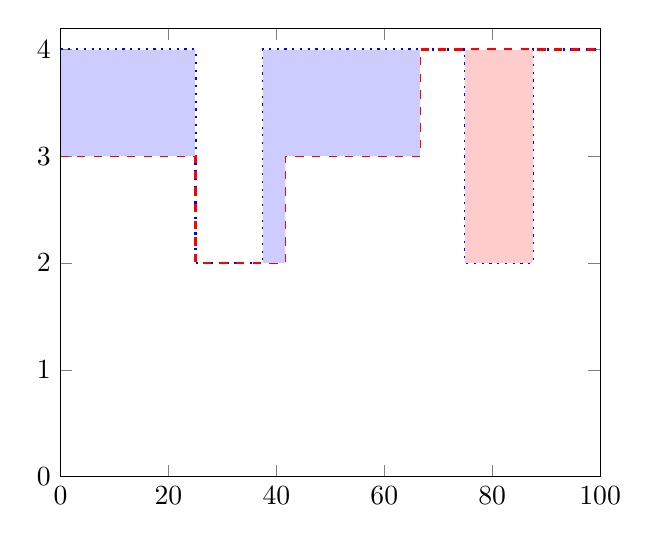
\begin{tikzpicture}
	\begin{axis}[ymin=0,ymax=4.2,enlargelimits=false]
	\addplot
	[const plot,blue, thick,dotted]
	coordinates
	{(0,    4) (25,    2) (37.5,    4) (75,    2) (87.5,    4) (100,    4)};
	\addplot
	[const plot, red, thick,style=dashed]
	coordinates
	{(0,    3) (25,    2) (41.6,    3) (66.66,    4) (100,    4)};
  \fill [blue,fill=blue!20] (axis cs:0,3) rectangle (axis cs:25,4);
	\fill [blue,fill=blue!20] (axis cs:37.5,2) rectangle (axis cs:41.6,3);
	\fill [blue,fill=blue!20] (axis cs:37.5,3) rectangle (axis cs:66.6,4);
	\fill [red,fill=red!20] (axis cs:75,2) rectangle (axis cs:87.5,4);
	\end{axis}
	\end{tikzpicture}
\caption{K�l�nb�z� hossz�s�g� ritmusok k�z�tti kronotonikus t�vols�g $100$ egys�g hossz� $x$ tengelyre vet�tve}
\label{fig:fig07}
\end{figure}

%----------------------------------------------------------------------------
\subsubsection{Szimmetria nem teljes�l�se eset�n}
%----------------------------------------------------------------------------

Ha �gy d�nt�nk, hogy a nem k�v�njuk megk�vetelni a szimmetria teljes�l�s�t, akkor rendelhet�nk k�l�nb�z� �rt�keket a r�videbb hosszabbt�l, illetve a hosszabb r�videbbt�l val� t�vols�g�rt�kek�nt. 

Tal�n nem t�ved�nk nagyot, ha egy r�videbb vektorra, melyet mag�ban foglal egy m�sik, azt mondjuk, hogy $0$ t�vols�gra van a hosszabbt�l. A hosszabb t�vols�ga a r�videbbt�l pedig annak f�ggv�ny�ben k�zel�t a $0$-hoz, hogy mekkora a k�z�tt�k l�v� hosszelt�r�s.

A nem szimmetrikus t�vols�gra n�zz�nk egy esetet, amelyn�l sz�m�t a sorrend $d_{H}(x,y)$ param�terez�s�ben (nevezz�k aszimmetrikus Hamming-t�vols�gnak).

A m�dszer sor�n nagyj�b�l az t�rt�nik, hogy a szumm�z�s el�tt a m�sodik vektort, amennyiben az r�videbb, mint az els�, null�kkal eg�sz�tj�k ki, hogy azonos hossz�ak legyenek. Ezek ut�n ugyan�gy vizsg�ljuk meg a kapott vektorok t�vols�g�t, mint az eredeti m�dszern�l.

Form�lisan, adott $X=(x_1,x_2,...,x_n)$ a n�la r�videbb $Y=(y_1,y_2,...,y_m)$-t�l val� t�vols�ga (teh�t $|X|=n$, $|Y|=m$, �s $n>m$):
\begin{align}
d_H(X,Y)=\sum_{i=1}^m |x_i-y_i|+ \sum_{i=m+1}^n |x_i|
\end{align}
hiszen a m�sodik tagban $0$-kat vonunk le az aktu�lis $x_i$-b�l.

Ezzel a m�dszerrel azt a val�s megfigyel�st realiz�lhatjuk, hogy ha egy $X$ vektor r�sze egy hosszabb $Y$-nak, akkor $d(X,Y)$ val�ban $0$, ezzel szemben $d(Y,X)$ nem felt�tlen�l egyenl� vele. Ha pedig ad�dik egy $X$-n�l hosszabb, $Y$-n�l m�g mindig r�videbb $Z$ vektor, mely szint�gy r�sze $Y$-nak, akkor $d(Z,X) \leq d(Y,X)$.

Az elj�r�s ugyan�gy �rtelmezhet� Manhattan-, �s Euklideszi-t�vols�gokra, de sajnos nem alkalmazhat� intervallum-k�l�nb�z�s�gi vektorok, cser�l�si t�vols�g �s kronotonikus l�ncok eset�n.
%----------------------------------------------------------------------------
\chapter*{K�sz�netnyilv�n�t�s}\addcontentsline{toc}{chapter}{K�sz�netnyilv�n�t�s}
%----------------------------------------------------------------------------

Ez nem k�telez�, ak�r t�r�lhet� is. Ha a szerz� sz�ks�g�t �rzi, itt lehet k�sz�netet nyilv�n�tani azoknak, akik hozz�j�rultak munk�jukkal ahhoz, hogy a hallgat� a szakdolgozatban vagy diplomamunk�ban le�rt feladatokat sikeresen elv�gezze. A konzulensnek val� k�sz�netnyilv�n�t�s sem k�telez�, a konzulensnek hivatalosan is dolga, hogy a hallgat�t konzult�lja.

%\listoffigures\addcontentsline{toc}{chapter}{�br�k jegyz�ke}
%\listoftables\addcontentsline{toc}{chapter}{T�bl�zatok jegyz�ke}

\bibliography{mybib}
\addcontentsline{toc}{chapter}{Irodalomjegyz�k}
\bibliographystyle{plain}

%----------------------------------------------------------------------------
\appendix
%----------------------------------------------------------------------------
\chapter*{F�ggel�k}\addcontentsline{toc}{chapter}{F�ggel�k}
\setcounter{chapter}{6}  % a fofejezet-szamlalo az angol ABC 6. betuje (F) lesz
\setcounter{equation}{0} % a fofejezet-szamlalo az angol ABC 6. betuje (F) lesz
\numberwithin{equation}{section}
\numberwithin{figure}{section}
\numberwithin{lstlisting}{section}
%\numberwithin{tabular}{section}

%----------------------------------------------------------------------------
\section{NEXUS f�jl p�lda}\label{app:nexus}
%----------------------------------------------------------------------------

\begin{lstlisting}[frame=single,captionpos=b,caption={A 21-es dallamoszt�lyhoz gener�lt Nexus f�jl (Hamming-t�vols�g alapj�n)}]
#NEXUS

BEGIN taxa;
	DIMENSIONS ntax=8;
TAXLABELS
	55
	315
	352
	723
	724
	1074
	1163
	1453
;
END;

BEGIN distances;
	DIMENSIONS ntax=8;
	FORMAT
		triangle=LOWER
		diagonal
		labels
		missing=?
	;
MATRIX
	55	0.000	
	315	0.125	0.000	
	352	0.475	0.431	0.000	
	723	0.370	0.370	0.524	0.000	
	724	0.523	0.523	0.692	0.415	0.000	
	1074	0.136	0.244	0.401	0.440	0.600	0.000	
	1163	0.190	0.298	0.401	0.480	0.644	0.045	0.000	
	1453	0.250	0.250	0.475	0.467	0.523	0.352	0.406	0.000	

;
END;
\end{lstlisting}

----------------------------------------------------------------------------
\clearpage\section{A m�sodik dallamoszt�ly szerkezete Hamming-t�vols�g alapj�n}\label{app:2ndcluster}
----------------------------------------------------------------------------

\vspace*{100px}

\begin{figure}[!h]
\centering
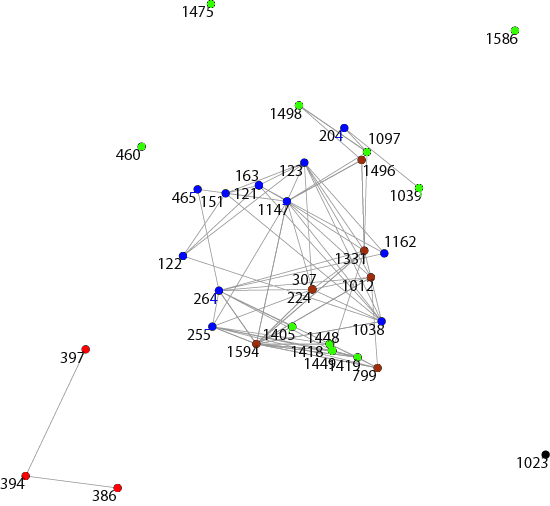
\includegraphics[width=120mm, keepaspectratio]{figures/cluster2MDS_kmeans.png}
\caption{A m�sodik dallamoszt�ly MDS �br�ja Hamming-t�vols�g alapj�n, k-means szerint sz�nezve} 
\end{figure}

\begin{figure}[!p]
\centering
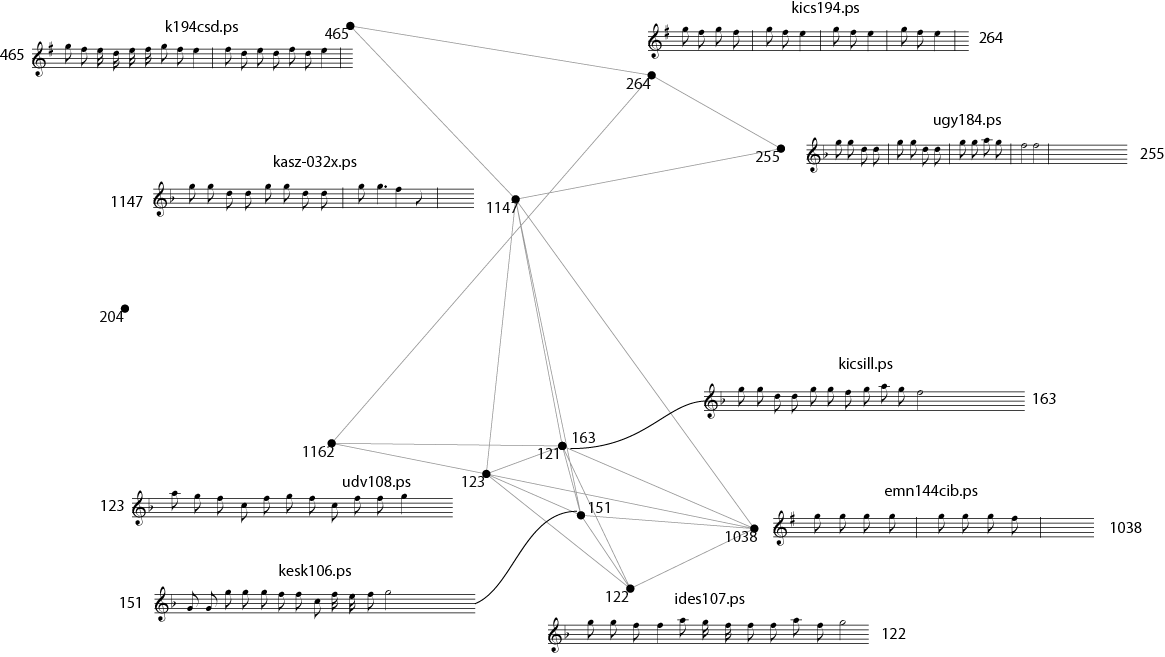
\includegraphics[width=150mm, keepaspectratio]{figures/cluster2furt1.png}
\caption{Els� klaszter: alul parlando keserves, fel�l 2*(4/4)-es �s 4*(2/4)-es v�ltozatok} 
\end{figure}

\clearpage

\begin{figure}[!p]
\centering
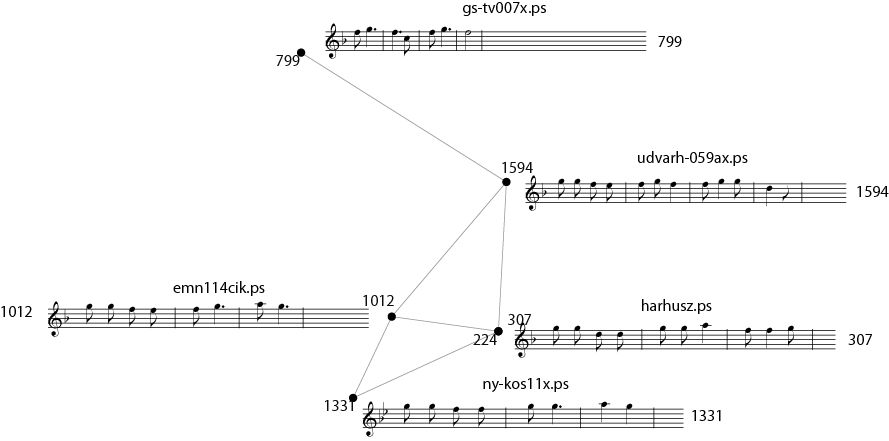
\includegraphics[width=150mm, keepaspectratio]{figures/cluster2furt2.png}
\caption{M�sodik klaszter: alul 3*(2/4), f�l�l 4*(2/4) - a b�v�l�s 224 �s 1594 k�z�tt t�rt�nik} 
\end{figure}

\clearpage

\begin{figure}[!p]
\centering
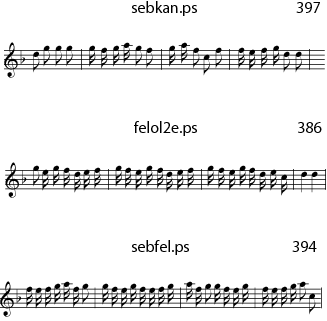
\includegraphics[width=80mm, keepaspectratio]{figures/cluster2furt3.png}
\caption{Harmadik klaszter: Hangszeres kan�szt�nc-t�pus v�ltozatai} 
\end{figure}

\clearpage

\vspace*{100px}

\begin{figure}[!h]
\centering
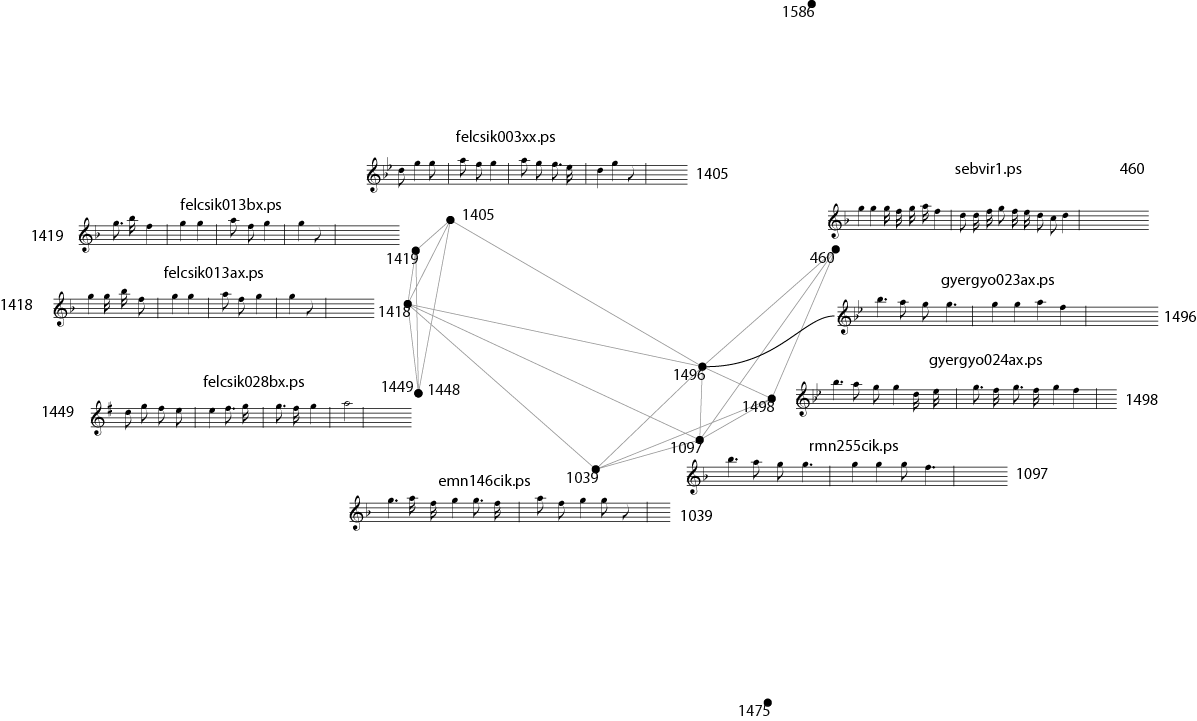
\includegraphics[width=150mm, keepaspectratio]{figures/cluster2furt4.png}
\caption{Negyedik klaszter: Bal oldalon 4*(2/4), jobb oldalon 2*(4/4)} 
\end{figure}

----------------------------------------------------------------------------
\clearpage\section{Az �t�dik dallamoszt�ly SplitsTree f�i k�l�nb�z� t�vols�gok alapj�n}\label{app:splits}
----------------------------------------------------------------------------

\vspace*{110px}

\begin{figure}[!h]
\centering
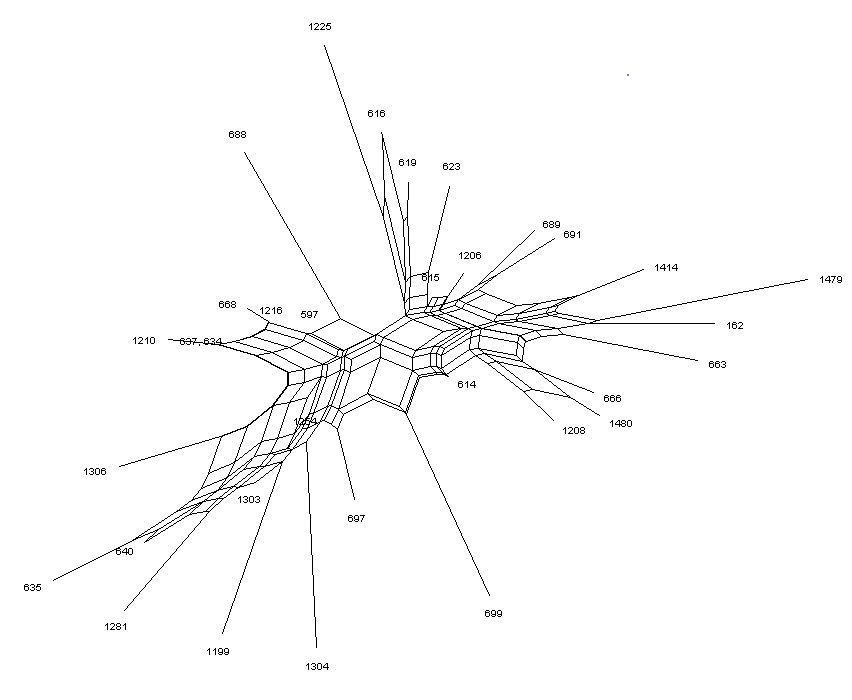
\includegraphics[width=150mm, keepaspectratio]{figures/cluster5_manhattan.png}
\caption{Az �t�dik dallamoszt�ly elemei Manhattan-t�vols�g alapj�n} 
\end{figure}

\begin{figure}[!p]
\centering
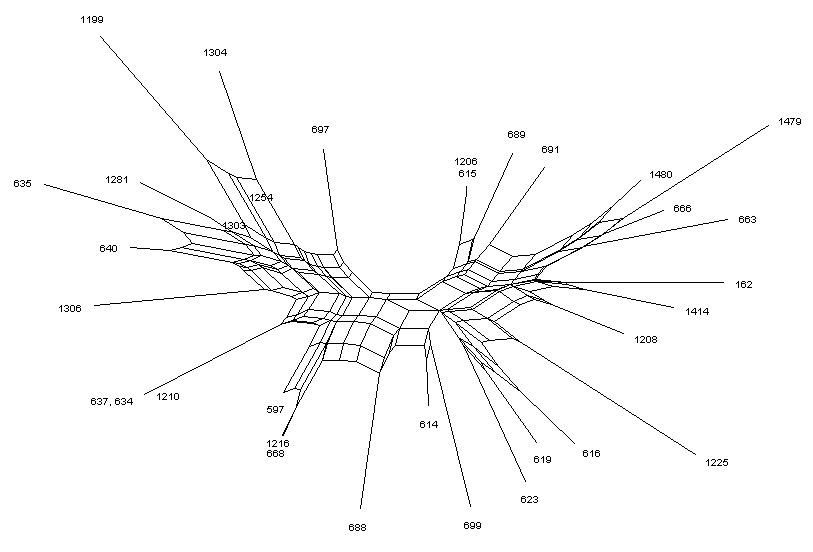
\includegraphics[width=150mm, keepaspectratio]{figures/cluster5_euclidean.png}
\caption{Az �t�dik dallamoszt�ly elemei Euklideszi-t�vols�g alapj�n} 
\end{figure}

\clearpage

\begin{figure}[!p]
\centering
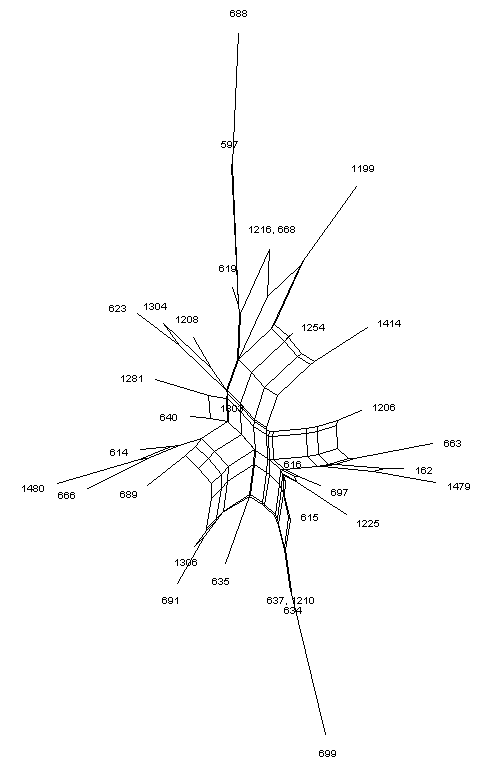
\includegraphics[width=110mm, keepaspectratio]{figures/cluster5_intervaldiff.png}
\caption{Az �t�dik dallamoszt�ly elemei intervallum-k�l�nb�z�s�gi vektorok t�vols�ga alapj�n} 
\end{figure}

\clearpage

\begin{figure}[!p]
\centering
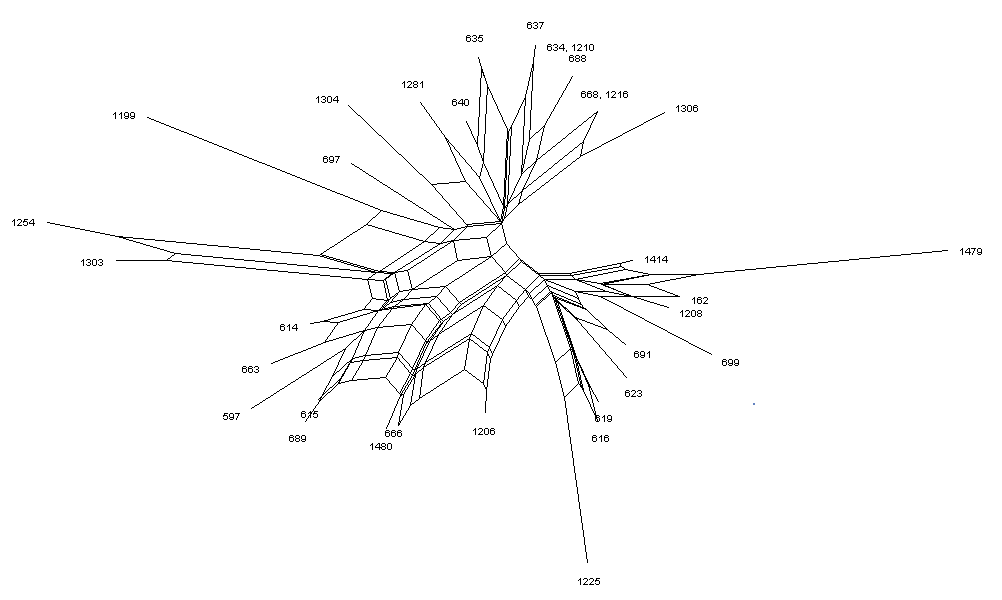
\includegraphics[width=150mm, keepaspectratio]{figures/cluster5_chronotonic.png}
\caption{Az �t�dik dallamoszt�ly elemei kronotonikus t�vols�g alapj�n} 
\end{figure}

\clearpage

\begin{figure}[!p]
\centering
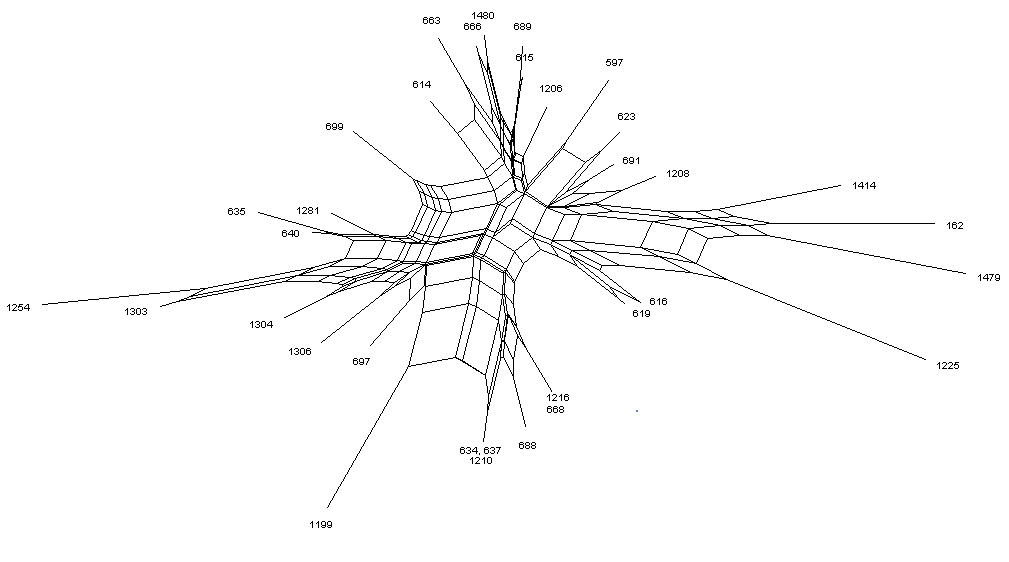
\includegraphics[width=150mm, keepaspectratio]{figures/cluster5_continouschronotonic.png}
\caption{Az �t�dik dallamoszt�ly elemei vet�tett kronotonikus t�vols�g alapj�n} 
\end{figure}

\clearpage

\begin{figure}[!p]
\centering
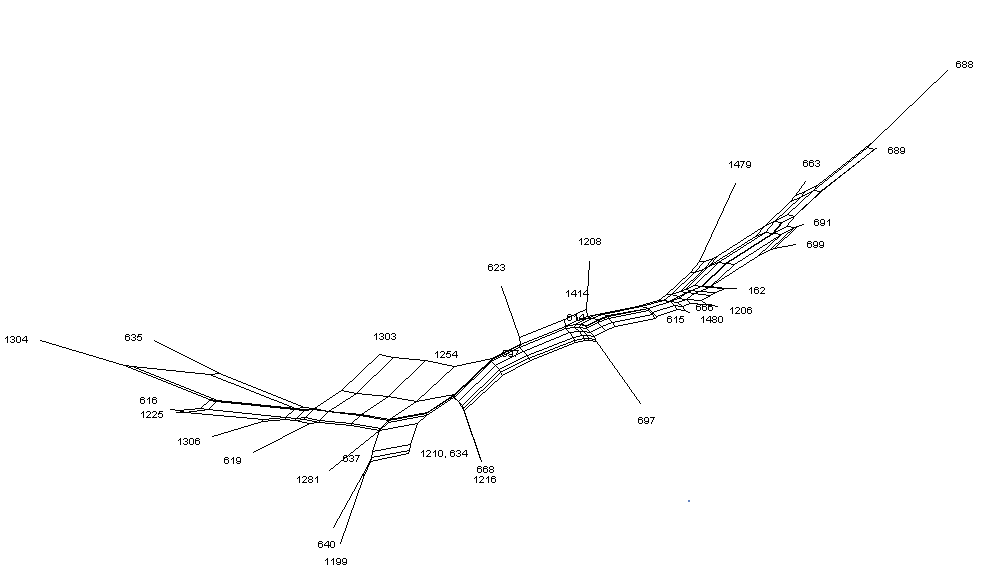
\includegraphics[width=150mm, keepaspectratio]{figures/cluster5_swap.png}
\caption{Az �t�dik dallamoszt�ly elemei cser�l�si t�vols�g alapj�n} 
\end{figure}


\label{page:last}
\end{document}
